\chapter{IMPLEMENTACI\'ON}
\section{Arquitectura de TariyKDD}
Para el desarrollo de TariyKDD se utilizaron computadores con procesador AMD 64 bits, disco duro Serial ATA,
\'util  al tomar los datos desde un repositorio y al momento de realizar pruebas de rendimiento de los
algoritmos, ya que su velocidad de transferencia es de 150 MB/sg; adem\'as la RAM que se utilizo fu\'e
superior a los 512 MB, ya que la Miner\'ia de Datos requiere grandes cantidades de memoria por el tama\~no de
los conjuntos de datos.\\

El sistema operativo sobre el cual se trabajo durante la implementaci\'on de TariyKDD es Fedora Core en su
versiones 3 y 5. El lenguaje de programaci\'on en el que esta elaborado TariyKDD es Java 5.0, 
actualizaci\'on 06.\\

Dentro del proceso de Descubrimiento de Conocimiento, TariyKDD comprende las etapas de Selecci\'on,
Preprocesamiento, Miner\'ia de Datos y Visualizaci\'on de Resultados. De esta forma la implementaci\'on de la
herramienta se hizo a trav\'es de los siguientes m\'odulos de software cuya estructura se muestra en la figura
\ref{arquitectura}.

\begin{figure}[!ht]
\centering
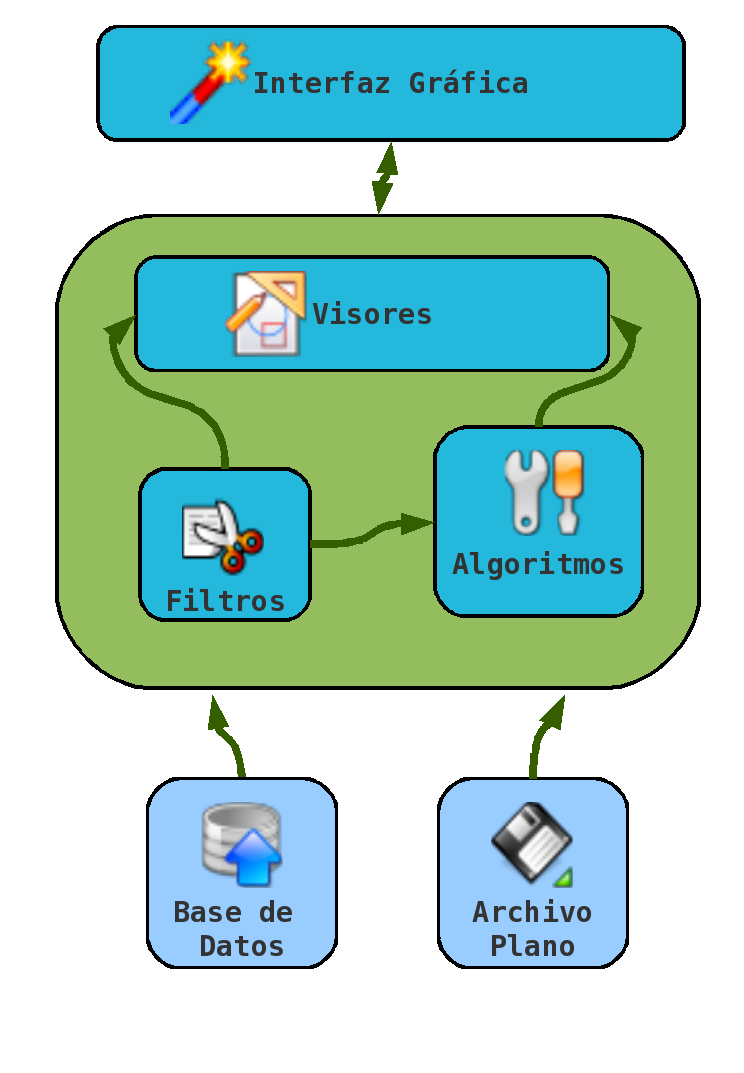
\includegraphics[width=0.35\textwidth]{images/arquitectura.png}
\caption{\'Arquitectura TariyKDD}
\label{arquitectura}
\end{figure}

%----------------------------------------- DESCRIPCION DE DESARROLLO --------------------------------------------%
\section{Descripci\'on del desarrollo de TariyKDD}
A continuaci\'on, en primera instancia se describe de manera general la estructura de TariyKDD para dar una idea
global de como esta herramienta fu\'e implementada. A continuaci\'on, se amplia y se detalla m\'as la forma en 
que TariyKDD fu\'e desarrollada.

\begin{itemize}
\item utils: Utilidades de TariyKDD. Dentro de este paquete encontramos clases como DataSet...
\item algorithm: Esta compuesta de los paquetes association y classification, los cuales implementan mediante sus
respectivas clases los algoritmos de asociaci\'on (Apriori, FPgrowth y EquipAsso) y clasificaci\'on (C4.5 y
MateBy).
\item gui: Comprende los paquetes Icons y KnowledgeFlow, los cuales a trav\'es de sus clases implementan la 
interfaz gr\'afica de la herramienta.
\end{itemize}
%------------------- PAQUETE UTILS
\subsection{Paquete Utils}
Esta clase esta compuesta por las siguientes clases:
\subsubsection{Clase AssocRules}

Esta clase es la encargada de generar reglas a partir de los \'arboles de itemsets frecuentes que generan los
algoritmos de asociaci\'on. Las reglas se generan teniendo en cuenta el par\'ametro \textit{confianza} . Los
atributos que maneja esta clase son los siguientes:\\

\textit{frequents }de tipo Vector: vector de \'arboles AVL que contienen  su ves itemsets frecuentes.\\

\textit{dictionary }de tipo ArrayList: arreglo que contiene los nombres de los itemsets frecuentes.\\

\textit{confidence }de tipo entero: variable en la que se especifica la confianza de evaluaci\'on de las reglas.\\

\textit{rules }de tipo ArrayList: arreglo en el que se almacenan las reglas que cumplan con la confianza.\\

El curso normal de los eventos empieza con el llamado al m\'etodo \textit{buildRules }en el cual se inicia el
recorrido del vector de de \'arboles AVL. La raiz de cada \'arbol es enviada como par\'ametro al m\'etodo
\textit{walkTree }que es el encargado de recorrer el \'arbol y armar por cada rama recorrida un arreglo que es
enviado al m\'etodo \textit{combinations }para que se generen todas las combinaciones posibles de esa rama y
obtener las nuevas reglas. Cada regla es evaluada para verificar que cumpla el nivel de confianza. La f\'ormula
para la evaluaci\'on de confianza es: $(soporte_Frecuentes / soporte_Antecedente) * 100$. Si una regla supera el
nivel de confianza es enviada al m\'etodo \textit{decodeFrecuents} para su decodificaci\'on. Al final para efectos
pr\'acticos de representaci\'on existen varios m\'etodos que permiten oredenar las reglas generadas de acuerdo a
varios par\'ametros: soporte, confianza u arden alfab\'etico.

\subsubsection{Clase AvlNode}
En esta clase se construye la estructura interna de datos de un nodo perteneciente a un \'arbol Avl. Los atributos
que maneja esta clase son los siguientes:\\

 \textit{element} de tipo ItemSet: aqui se guardan los datos con los que se carga el nodo.\\

 \textit{left, right} de tipo Avlnode: punteros hacia los hijos izquierdo y derecho respectivamente.\\

 \textit{height} de tipo entero: altura del \'arbol Avl.\\

 \textit{check} de tipo booleano: variable de control del balance del \'arbol.

\subsubsection{Clase AvlTree}

Esta clase es la encargada tanto de crear o armar un arbol Avl como de proveer los m\'etodos necesarios para su
manejo. Un \'arbol Avl es un tipo de \'arbol binario que es balanceado de tal manera que la profundidad de dos
hojas cualquiera en el \'arbol difiera como m\'aximo en uno. Los atributos de esta cln los siguientes:\\

 \textit{root} de tipo Avlnode: raiz del \'arbol Avl\\

 \textit{n} de tipo entero: variable de control de la profundidad o n\'umero de niveles del \'arbol.\\

 \textit{node} de tipo AvlNode: nodo para recorrer el \'arbol.\\

 \textit{stack} de tipo Stack: pila utilizada para almacenar la ruta del recorrido hecho en una inserci\'on,
 b\'usqueda o eliminaci\'on.\\

Para lograr la construcci\'on y manejo de un \'arbol Avl son necesarios algunos m\'etodos, los cuales ser\'an
mencionados m\'as no explicados debido a su complejidad y a que estos m\'etodos son bastante conocidos dentro del
\'ambito de las estructuras de datos. Los m\'etodos implementados son: \textit{insert, find, height,
rotateWithLeftChild, rotateWithRightChild, doubleWithLeftChild, doubleWithRightChild}, m\'etodos de inserci\'on,
b\'usqueda, consulta de profundidad del \'arbol, rotaci\'on por el hijo izquierdo, rotaci\'on por el hijo derecho,
doble rotaci\'on por izquierda y doble rotaci\'on por derecha respectivamente.

\subsubsection{Clase BaseDatos}
Esta clase es utilizada siempre que se necesite efectuar conexiones a bases de datos por medio del objeto de
conexi\'on java para Postgres. Cabe aclarar que el sistema gestor de bases de datos (SGBD) inicial es Postgres pero
el nombre del sistema gestor es totalmente parametrizable, permitiendo de esta manera la conexi\'on a casi
cualquier SGBD. Los atributos de esta clase son:\\

 \textit{db} de tipo Connection: objeto encargado de establecer la conexi\'on.\\

 \textit{stm} de tipo Statement: variable encargada de ejecutar un query determinado.\\

 \textit{nombre} de tipo String: nombre de la base de datos.\\

Inicialmente se estable el nombre del contolador de la base de datos que se desea consultar. En este caso el
controlador Postgres. Luego se llama al m\'etodo \textit{iniciarBD} que se encarga de establecer la conexi\'on a la
base de datos. Tiene como par\'ametros el nombre de la base de datos, el nombre del usuario y constrase\~na.\\

Existen otros m\'etodos implementados para la consulta del nombre de las tablas, inserci\'on y consulta de los
datos de una tabla. El m\'etodo \textit{getTablas} retorna un vector con los nombres de las tablas que contenga la
base de datos. El m\'etodo \textit{insertarBD} permite insertar un registro nuevo en una tabla. Tiene como
par\'ametros el nombre de la tabla, el identificador de u item y el nombre del item a insertar.  \textit{getDatos}
permite ejecutar una consulta general a una tabla. Solo requiere el nombre de la tabla a consultar.

\subsubsection{Clase FileManager}

Esta clase se encarga de todo lo que tiene que ver con el manejo de archivos de acceso a aleatorio y el flujo de
informaci\'on entre el archivo le\'ido, el DataSet y el diccionario de datos. 
Los atributos de esta clase son:\\

 \textit{out} de tipo File: archivo al cual se va a leer o escribir.\\

 \textit{outChannel} de tipo RandomAccessFile: puntero para ubicarse en el archivo de acceso aleatorio. Proporciona
 el flujo hacia el archivo.\\

 \textit{data} de tipo Object: matriz con los datos de un archivo de acceso aleatorio .arff\\

 \textit{attributes} de tipo Object: arreglo con los nombres de los atributos de un archivo de acceso aleatorio
 .arff.\\

 \textit{dictionary} de tipo Array List: arreglo en el que se almacena el diccionario de datos de un archivo
 .arff\\

 Dentro de la lista de utilidades que se pueden encontrar en esta clase se pueden listar las siguientes:\\

 \textit{writeItem}: m\'etodo utilizado para escribir un entero corto (short) en un archivo. C\'odigo \ref{c2}\\

\begin{codigof}[t]
\begin{verbatim}
...
  public void writeItem(short s) {
  try{
    outChannel.seek( out.length() );
    outChannel.writeShort(s);
  } catch( IOException e ) {
  e.printStackTrace();
  }
  }
...
\end{verbatim}
\caption{Escribir un item a archivo}
\label{c2}
\end{codigof}

\textit{writeString}: m\'etodo utilizado para escribir una cadena de caracters en un archivo. C\'odigo \ref{c3}.

\begin{codigof}[!h]
\begin{verbatim}
...
  public void writeString(String s){
  byte b[];
  try{
    b = s.getBytes();
    outChannel.seek( out.length() );
    outChannel.write(b);
  } catch( IOException e ) {
  e.printStackTrace();
  }
  }
...
\end{verbatim}
\caption{Escribir una cadena a archivo}
\label{c3}
\end{codigof}

\textit{getFileSize}: retorna el tama\~no de un archivo en bytes. Cuadro \ref{c4}\\

\begin{codigof}[!h]
\begin{verbatim}
...
  public long getFileSize() {
  return out.length();
  }
...
\end{verbatim}
\caption{Tama\~no de un archivo}
\label{c4}
\end{codigof}

 \textit{getFileName}: retorna el nombre del archivo de acceso aleatorio. Cuadro \ref{c5}\\

\begin{codigof}[t]
\begin{verbatim}
...
  public String getFileName() {
  return out.getName();
  }
...
\end{verbatim}
\caption{Nombre de un archivo}
\label{c5}
\end{codigof}

 \textit{closeFile}: cierra el flujo hacia el archivo de acceso aleatorio. Cuadro \ref{c6} \\

\begin{codigof}[h]
\begin{verbatim}
...
  public void closeFile() {
  try{
    outChannel.close();
  } catch(IOException e) {
  e.printStackTrace();
  }
  }
...
\end{verbatim}
\caption{Cierra conexi\'on a archivo}
\label{c6}
\end{codigof}
 \textit{deleteFile}: borra f\'i{}sicamente el archivo de acceso aleatorio. \ref{c7} \\

\begin{codigof}[h]
\begin{verbatim}
...
  public void deleteFile() {
  out.deleteOnExit();
  }
...
\end{verbatim}
\caption{Borrar un archivo}
\label{c7}
\end{codigof}

 \textit{setOutChannel}: ubica el flujo en una posici\'on determinada del archivo de acceso aleatorio.
C\'odigo \ref{c8}.\\

\begin{codigof}[t]
\begin{verbatim}
...
  public void setOutChannel(int pos) throws IOException {
  outChannel.seek(pos);
  }
...
\end{verbatim}
\caption{Manejo de posici\'on en un archivo}
\label{c8}
\end{codigof}

\textit{ReadTransaction}: lee y muestra el contenido de un archivo de acceso aleatorio. Esta funci\'on
es \'util para el antiguo formato de archivos Tariy, lee un flujo de tipo \textit{Short }y muestra cada
transacci\'on separada por el cero. C\'odigo \ref{c9}\\

\begin{codigof}[!h]
\begin{verbatim}
...
  public void ReadTransaction(int readposition) {
  try{
    outChannel.seek(readposition);
    short s;
    while( true ) {
    s = outChannel.readShort();
    if(s != 0)
      System.out.print(s + " ");
    else
      System.out.println();
    }
  } catch(EOFException e1) {
    this.closeFile();
  } catch(IOException e2) {
    e2.printStackTrace();
  }
  }
...
\end{verbatim}
\caption{Lectura de un archivo}
\label{c9}
\end{codigof}

\textit{getAttributes}: retorna el arreglo que tiene los nombres los atributos del archivo de acceso
aleatorio .arff. C\'odigo \ref{c10} \\

\begin{codigof}[!h]
\begin{verbatim}
...
  public Object[] getAttributes() {
  return attributes;
  }
...
\end{verbatim}
\caption{Nombres de atributos de un archivo plano}
\label{c10}
\end{codigof}

\textit{getData}: retorna la matriz que almacena los datos del archivo de acceso aleatorio .arff. C\'odigo
\ref{c11} \\

\begin{codigof}[t]
\begin{verbatim}
...
  public Object[][] getData() {
  return data;
  }
...
\end{verbatim}
\caption{Matriz de datos del archivo plano}
\label{c11}
\end{codigof}

 \textit{getDictionary}: retorna el diccionario de datos construido a partir del archivo de acceso
aleatorio .arff. \\

 \textit{buildMultivaluedDataset}: este es uno de los m\'etodos m\'as importantes en la face de carga de
los datos desde el archivo plano a memoria. El archivo de extenci\'on arff se recorre completamente pero solo se
cargan los datos necesarios al DataSet. Por ejemplo, en un archivo arff se pueden encontrar algunas etiquetas
propias como lo son \textit{@data }y \textit{@attribute}. Este tipo de etiquetas son ignoradas al igual que los
espacios en blanco. Debido a que el objetivo es tratar de ahorrar espacio en memoria y a la naturaleza del DataSet
los datos del archivo plano no pueden ser almacenados directamente como vienen. Los datos se codifican como
enteros cortos \textit{shorts} y sus nombres originales se almacenan en un diccionario para poder recuperarlos en
el proceso inverso en el momento de generar las reglas.\\

 \textit{buildUnivaluedDataSet}: este es un m\'etodo similar al anterior pero optimizado para manejar
archivos univaluados, es decir, aquellos que solo tienen dos columnas una de las cuales es el identificador y la
otra el nombre del art\'iculo.\\

 \textit{dataAndAttributes}: a partir de un archivo de acceso aleatorio .arff, almacena los nombres de
los atributos en un arreglo, los datos en una matriz y el diccionario de datos en un ArrayList.\\

 \textit{builtDataMatrix}: retorna una matriz que representa un archivo de acceso aleatorio .arff con los
nombres de sus atributos y sus datos.\\ \\

 \textbf{Clase ItemSet}\\

 Esta clase se encarga del manejo de los conjuntos de items. Un itemSet puede ser entendido como una
trasacci\'on. Los atributos de esta clase son:\\

 \textit{items} de tipo short: arreglo que almacena los items que forman el itemset.\\

 \textit{support} de tipo short: soporte asociado a este itemset.\\

 \textit{n} de tipo short: tama\~no del itemset.\\

 Los m\'etodos implementados son:\\

 \textit{getItems}: retorna el item asociado.\\

 \textit{getSupport}: retorna el soporte de un itemset\\

 \textit{gettype}: retorna el tipo de un itemset, el tipo se deriva del tama\~no del itemset.\\

 \textit{setSupport}: establece el soporte de un itemset.\\

 \textit{increaseSupport}: incrementa el soporte de un itemset, ya sea en uno o el n\'umero que se
requiera.

\subsubsection{Clase NodeNoF}
Esta clase se encarga de crear los nodos intermedios de un \'arbol de datos. Tambi\'en se implementan
los m\'etodos para enlazar un nodo a otro. Entre ellos se encuentran: addSon, addBro y findBro que se encargan de
adicionar un hijo, adicionar un hermano y buscar si un nodo tiene hermanos respectivamente.

\subsubsection{Clase NodeF}
Esta clase extiende a la clase NodeNoF. este tipo de nodos son las hojas de las ramas. Lo que las hace
diferentes, son dos atributos adicionales, uno es el soporte, que se encarga de llevar a cabo el conteo de veces
que una transacci\'on repetida ha sido tenida en cuenta, y el otro es un puntero a otra hoja. En el momento de
recorrer un \'arbol, el tipo de nodo nos permite saber que hemos llegado al final de una rama.

\subsubsection{Clase Transaction}
Esta clase es la encargada de manejar los itemsets o conjuntos de items por cada transacci\'on. Cada uno
de los itemsets son almacenados en vectores. Esta clase se encarga de alimentar esos vectores, permite hacer
consulta sobre ellos u organizarlos. Estos m\'etodos se muestran a continuaci\'on:\\

 \textit{getArticles}: permite ver los articulos en una transacci\'on.\\

 \textit{getSize}: devuelve el tama\~no de una transacci\'on.\\

 \textit{getItemset}: devuelve un item de la trnsacci\'on.\\

 \textit{srtBySupport}: ordena las transacciones por soporte.\\

 \textit{srtByItem}: ordena las transacciones por el item.\\

 \textit{loadItemsets}: carga los art\'iculos o items de una transacci\'on.\\

 \textit{clearTransaction}: borra los items de una transacci\'on.\\

%------------------- PAQUETE ALGORITHM
\subsection{Paquete algorithm}
Este paquete esta compuesto a su vez por los paquetes association y classification, los cuales implementan los 
algoritmos de Asociaci\'on (Apriori, FPgrowth y EquipAsso) y Clasificai\'on (C4.5 y MateBy).

%------------------- PAQUETE ASSOCIATION
\subsubsection{Paquete association}
El paquete association esta conformado por los paquetes que implementan los algoritmos de asociaci\'on y que se
explican a continuaci\'on:

%------------------- PAQUETE APRIORI
\paragraph{Paquete Apriori}
La implementaci\'on del algoritmo apriori se realiz\'o utilizando una clase denominada apriori.java que
interactua directamente con otras clases definidas en el paquete Utils como DataSet, Transaction, AvlTree e
Itemset.  Al igual que las otras clases que implementan algoritmos de asociaci\'on, en el constructor de la clase
Apriori se usan 2 parametros:  una instancia de la clase DataSet, donde vienen comprimidos el conjunto de datos
desde el m\'odulo de conexi\'on o el m\'odulo de filtros, y un entero corto, que es suministrado por el usuario,
que ser\'a usado como el soporte del sistema durante la ejecuci\'on de este algoritmo.\\

De igual manera, en la construcci\'on de la clase se instancia e inicializa un objeto de la clase AvlTree que
almacenar\'a los itemsets frecuentes tipo 1, el cual es alimentado haciendo uso del m\'etodo
\textit{pruneCandidatesOne} de la clase DataSet, el cual recibe el soporte del sistema como parametro.  En este
punto tambi\'en se instancia e inizializa  un arreglo que guardar\'a los diferentes \'arboles balanceados
(AvlTree), que contendr\'an los Itemsets Frecuentes de cada tipo y que ser\'an calculados por la herramienta. Al
disponer ya de los itemsets frecuentes tipo 1, estos son almacenados en la posicion 0 de este arreglo.  Los
detalles del constructor de esta clase se aclaran en el siguiente listado:\\

\begin{codigof}[h]
\begin{verbatim}

public Apriori(DataSet dataset, short support) {
  this.support = support;
  this.dataset = dataset;
  AvlTree frequentsOne = new AvlTree();
  frequentsOne = dataset.pruneCandidatesOne(support);
  Trees.addElement(frequentsOne);
  auxTree = frequentsOne;
}
\end{verbatim}
\caption{Constructor de la clase \textit{Apriori}}
\end{codigof}

Para disparar la ejecuci\'on del algoritmo usamos el m\'etodo \textit{run} el cual ejecuta un ciclo dentro del
cual el m\'etodo \textit{makeCandidates} se encarga de generar todos los itemset candidatos para cada
iteraci\'on.  Para esto el m\'etodo \textit{makeCandidates} llama al objeto \textit{auxTree}, instancia de la
clase AvlTree que conserva el ultimo \'arbol de itemset frecuentes y pregunta cuantos itemsets tiene en ese
instante utilizando el m\'etodo \textit{howMany} de esta clase.\\

Para cada elemento encontrado dentro del \'arbol de Itemsets Frecuentes se recorre un ciclo con los dem\'as
miembros del \'arbol armando combinaciones que generan un nuevo itemset candidato haciendo uso del m\'etodo
\textit{combinations} que recibe como parametros el \'arbol \textit{auxTree} de Itemset Frecuentes y un \'arbol
AvlTree donde se guardaran los Itemsets Frecuentes tipo k + 1 llamando \textit{frequents}.  Se aprovecha la
ventaja de que los itemsets est\'an ordenados en el \'arbol y se verifica que el itemset evaluado coincida en sus
$n-1$ primeros items, siendo $n$ el tama\~no de ese itemset, con el proximo itemset del \'arbol. De ser as\'i, se
instancia un nuevo itemset con los $n-1$ items coincidentes y los 2 \'ultimos items de cada itemset involucrado. 
De esta manera se generan itemsets candidatos de tama\~no $n+1$.\\

Cada itemset candidato es pasado como par\'ametro al m\'etodo \textit{increaseSupport} donde es contado el
n\'umero de ocurrencias de ese itemset candidato dentro del conjunto de datos.  En este punto se hace una
consideraci\'on importante y si los itemsets candidatos que se est\'an construyendo son de tipo 3 o superior se
evalua el paso de poda, esto es, se descompone el itemset candidato construido en sus $n-2$ posibles
combinaciones del tipo anterior, siendo $n$ el tama\~no del itemset candidato que se esta generando.  No se
evaluan las dos \'ultimas combinaciones pues fueran estas las que generaron el candidato que se esta analizando y
se tiene certeza de que existen en el \'arbol de Itemsets Frecuentes.  Cada una de las combinaciones generadas
son buscadas en \textit{auxTree}, hay que recordar que este es el \'arbol que contiene todos los Itemsets
Frecuentes del orden anterior al que se esta generando.  Si una de las combinaciones del itemset candidato actual
no es encontrada en el \'arbol \textit{auxTree}, este itemset ya no es considerado y se procede a evaluar el
pr\'oximo.  El m\'etodo \textit{pruneCandidate} se encarga de realizar este an\'alisis y se presenta en el
cuadro \ref{codapri2}.\\

\begin{codigof}[ht]
\begin{verbatim}

private boolean pruneCandidate(ItemSet candidate) {
  int size = candidate.size;
  ItemSet auxiliar;
  for(int i = 0; i < size - 2; i++) {
  aux = new ItemSet(size - 1);
  int k = 0;
  for(int j = 0; j < size; j++) {
    if(j != i) {
    auxiliar.addItem(candidate.getItems()[j]);
    }
  }
  if(auxTree.findItemset(auxiliar) == null) {
    return false;
  }
  }
  return true;
}
\end{verbatim}
\caption{Funci\'on \textit{pruneCandidates}}
\label{codapri2}
\end{codigof}

Si el itemset candidato actual es de tipo 2 o ha superado el paso de poda se proceder\'a a hacer su conteo.  Para
ello, se hace una nueva instancia de la clase \textit{Transaction} donde se carga una a una las transacciones del
conjunto de datos y se compara con el contenido del itemset.  Si coinciden los elementos del registro y el
itemset, este \'ultimo incrementa su soporte interno en uno.\\

Al final de este proceso se cuenta con un itemset candidato con su soporte establecido, este se compara con el
soporte del sistema y de superarlo es incluido en el \'arbol \textit{frequents}.  Cuando ya se han evaluado todos
los candidatos para un \'arbol \textit{auxTree}, se pregunta si se han generado nuevos Itemsets Frecuentes en
\textit{frequents}.  Si el m\'etodo \textit{howMany} de \textit{frequents} arroja existencias se almacena en el
arreglo de  \'arboles frecuentes y se asigna a \textit{auxTree} el \'arbol \textit{frequents} para iniciar de 
nuevo el proceso de generaci\'on de candidatos.  Esto se har\'a hasta que el \'arbol \textit{frequents} resulte
vac\'io (no hayan nuevos Itemsets Frecuentes).  En el arreglo de \'arboles frecuentes quedan almacenados todos
los Itemsets Frecuentes organizados por tipo que ser\'an pasados al M\'odulo de visores para ser visualizados
como reglas.
%------------------- PAQUETE FPGROWTH
\paragraph{Paquete FPgrowth}
Las clases que implementan el algoritmo FPgrowth se encuentran agrupadas en el paquete con el mismo nombre y las
m\'as importantes para su funcionamiento son FPGrowth, FPGrowthNode, FrequentNode, BaseConditional, 
BaseConditionals, Conditionals y AvlTree.\\

Tal y como se puede ver en la secci\'on \ref{fpgrowth}, el algoritmo FP-growth se basa en la generaci\'on de
itemsets candidatos a partir de un \'arbol N-Ario. Para comprender mejor la implementaci\'on de FP-growth, se
deben revisar primero las clases que forman la estructura del \'arbol N-Ario, las cuales han sido llamadas
FrequentNode y FPGrowthNode.

\subparagraph{Clase FrequentNode}
Para la posterior creaci\'on de itemsets frecuentes se almacenan en un array de objetos de tipo FrequentNode los
itemsets frecuentes-1 o de tama\~no 1. Cada uno de los items frecuentes-1 de esta lista se encuentra enlazado a
un nodo del \'arbol N-ario, de ahora en adelante FPtree, que tenga el mismo nombre que el itemset frecuente-1.

\subparagraph{Clase FPGrowthNode}
Esta clase proporciona la estructura del FPtree, en donde cada nodo tiene un valor de item, un soporte y los
punteros respectivos para realizar los enlaces entre nodos (Punteros al nodo hijo, al nodo padre, al nodo
hermano y al siguiente nodo con el mismo nombre). Su estructura se puede ver en el cuadro \ref{codfpgr1}.\\

\begin{codigof}[!h]
\begin{verbatim}

Atributos:
  short item //Dato que se va a a\~nadir al FPtree.
  short support //Soporte del item a\~nadido.
  FPGrowthNode fat //Puntero al nodo padre.
  FPGrowthNode son //Puntero al nodo hijo.
  FPGrowthNode bro //Puntero al nodo hermano.
  FPGrowthNode next //Puntero al siguiente nodo con el mismo valor.
\end{verbatim}
\caption{Estructura \textit{FPGrowthNode}}
\label{codfpgr1}
\end{codigof}

\subparagraph{Clase FPGrowth}
FPGrowth es la clase principal del paquete, tiene los m\'etodos m\'as importantes del algoritmo y a trav\'es
de los cuales se obtienen los itemsets frecuentes. Su estructura se puede ver en el cuadro \ref{codfpgr2}.\\

\begin{codigof}[ht]
\begin{verbatim}

Atributos:
  DataSet dataset //Estructura que comprime el conjunto de datos.
  short support //Soporte con el que se van a evaluar los datos.
  FrequentNode[] frequentsOne //Array que almacena a los itemsets 
  			    //frecuentes-1.
  FPGrowthNode cab //Raiz del FPtree.
  Vector Trees //Almacena los itemsets frecuentes de todos los 	
  	     //tamanos.
\end{verbatim}
\caption{Estructura \textit{FPGrowth}}
\label{codfpgr2}
\end{codigof}

Los parametros que el algoritmo FP-growth recibe en su constructor son, DataSet y el soporte suministrado por el
usuario. El primer paso de la implementaci\'on de FPGrowth es crear la lista con los itemsets frecuentes-1, la
cual se almacena en el array frequentsOne. El siguiente paso es construir el FPtree, para esto se lee cada una de
las transacciones de DataSet y para aquellos items cuyo soporte sea mayor o igual al m\'inimo se los almacena en
la clase del paquete Utils \textit{Transaction}. A partir de estos items filtrados se construye el FPtree, cuyo
seudoc\'odigo se puede observar en el cuadro \ref{codfpgr3}.\\

\begin{codigof}[!h]
\begin{verbatim}

boolean comienzo = true
puntero_referencia = null
do while (!fin de DataSet)
  transaccion_filtrada = transaccion(i)
  si (comienzo)
  Crear raiz de FPtree
  comienzo = false
  end si
  while (!fin de transaccion_filtrada)
  si (puntero_referencia == null)
    anadir nuevo_nodo como hijo
  end si
  si_no
  si (puntero_referencia = nuevo_nodo)
    incrementar_soporte ultimo_nodo
  end si
  si_no
    while(puntero_referencia tenga hermanos)
    si (nodo_hermano = nuevo_nodo)
      incrementar_soporte nodo_hermano
      terminar while
    end si
    end while
    si (puntero_referencia no tiene mas hermanos)
    anadir nuevo_nodo como hermano
    end si
  end while
end do
\end{verbatim}
\caption{Seudocodigo construcci\'on \textit{FPtree}}
\label{codfpgr3}
\end{codigof}

Para una mejor compresi\'on sobre la construcci\'on del FPtree se puede observar el conjunto de datos del cuadro
\ref{datos1} y su representaci\'on gr\'afica en la figura \ref{arbolfptree} y para profundizar m\'as en la
implementaci\'on se puede observar en el cuadro \ref{codfpgr4} el c\'odigo fuente de la funci\'on que construye el
FPtree (\textit{buildTree}):\\

\newpage
\begin{codigof}[!h]
\begin{verbatim}
  
  short frequent;
  BaseConditional baseconditional;
  BaseConditionals bcs;
  Vector path = new Vector(1,1);
  aux = cab.son;
  FPGrowthNode pcb, pcab;
  Arrays.sort(frequentsOne, new compareFrequentNode());
  for(int i = frequentsOne.length - 1; i >= 0; i--){
    FrequentNode aux = (FrequentNode) frequentsOne[i];
    pcb = aux.pcab;
    pcab = aux.pcab;
    frequent = pcb.getItem();
    bcs = new BaseConditionals(frequent, support);
    while(pcab != null){
    path.clear();
    pcb = pcb.fat;
    while(pcb != null){
      path.add((short) pcb.getItem());
      pcb = pcb.fat;
    }
    if(path.size() != 0){
      baseconditional = new BaseConditional(path, 
	          pcab.getSupport());
      bcs.addBaseConditionals(baseconditional);
    }
    pcab = pcab.next;
    pcb = pcab;
    }
    bcs.sortByElement();
    Trees = bcs.buildConditionals(Trees);
  }
\end{verbatim}
\caption{Funci\'on \textit{buildTree}}
\label{codfpgr4}
\end{codigof}

\newpage
\begin{table}[!h]
\begin{center}
\begin{tabular}{|p{25mm}|p{35mm}|}\hline
\textbf{Transacci\'on} & \textbf{Lista de items}\\ \hline\hline
T01 & \{(1,2,5)\}\\ \hline
T02 & \{(2,4)\}\\ \hline
T03 & \{(2,3)\}\\ \hline
T04 & \{(1,2,4)\}\\ \hline
T05 & \{(1,3)\}\\ \hline
T06 & \{(2,3)\}\\ \hline
T07 & \{(1,3)\}\\ \hline
T08 & \{(1,2,3,5)\}\\ \hline
T09 & \{(1,2,3)\}\\ \hline
\end{tabular}
\end{center}
\caption{Conjunto de datos transaccional}
\label{datos1}
\end{table}

\begin{figure}[!h]
\centering
\includegraphics[width=0.8\textwidth]{images/fptree.png}
\caption{\'Arbol FPtree}
\label{arbolfptree}
\end{figure}

Como se puede observar en la figura \ref{arbolfptree}, cada uno de los items frecuentes-1 se encuentra enlazado a
un nodo del FPtree, por ejemplo el item frecuente-1, 5 se encuentra enlazado al nodo de FPtree 5, cuyo soporte es
1 y a la vez cada nodo de FPtree se enlaza al siguiente nodo con el mismo nombre, en el caso del nodo 5, este se
enlaza a otro nodo con valor 5 y cuyo soporte es 1.\\

El siguiente paso de la implementaci\'on cosiste en recorrer la estructura de los items frecuentes-1 y por cada
uno de estos construir sus Patrones Condicionales Base, los cuales se obtienen recorriendo FPtree desde cada nodo
enlazado por los items frecuentes-1 a trav\'es de su puntero al nodo padre hasta la raiz. Por ejemplo como se
puede observar en la figura \ref{arbolfptree} para el item frecuente-1, 5 sus Patrones Condicionales Base son
dos: (1,2:1) y (3,1,2:1), donde el n\'umero despu\'es de '':'' es el soporte del Patr\'on, el cual corresponde al
mismo soporte que tenga el item frecuente-1 en cuestion. Cada uno de los Patrones Condicionales Base se almacenan
en la clase \textit{BaseConditional} y todo el conjunto de Patrones Condicionales Base de un item frecuente-1 se
alamcenan en la clase \textit{BaseConditionals}. En el cuadro \ref{pcb} se pueden observar los Patrones
Condicionales Base de cada uno de los items frecuentes-1.\\

Cuando se han construido todos los Patrones Condicionales Base de un item frecuente-1, el siguiente paso de la
implementaci\'on es determinar cuales de sus items tienen soporte mayor o igual al m\'inimo. Para esto se debe 
sumar cada uno de los soportes que un item tenga en cada Patr\'on Condicional Base, los items que cumplan con el
soporte van a conformar los Patrones Condicionales, los cuales se almacenan en la clase \textit{Conditionals},
por ejemplo para un soporte m\'inimo igual a 2 los Patrones Condicionales del item frecuente-1 son (1:2) y (2:2),
se puede observar que el item 3 no cumple con el soporte, por tanto no es Patr\'on Condicional. Los Patrones
Condicionales de los items frecuentes-1 se pueden observar en el cuadro \ref{pcb}.\\

\begin{table}[h]
\begin{center}
\begin{tabular}{|p{9mm}|p{35mm}|p{30mm}|p{40mm}|}\hline
\textbf{Item} & \textbf{Patrones Condicionales Base} & \textbf{Patrones Condicionales} & \textbf{Patrones
Frecuentes}\\ \hline\hline
5 & \{(1,2:1),(3,1,2:1)\}   & (2:2, 1:2)     & (2,5:2),(1,5:2)(2,1,5:2)\\ \hline
4 & \{(2:1),(1,2:1)\}     & (2:2)      & (2,4:2)\\ \hline
3 & \{(2:2),(1:2),(1,2:2)\} & (2:4, 1:2),(1:2) & (2,3:4),(1,3:2),(2,1,3:2)\\ \hline
1 & \{(2:4)\}         & (2:4)      & (2,1:4)\\ \hline
\end{tabular}
\end{center}
\caption{Patrones Condicionales e Itemsets Frecuentes}
\label{pcb}
\end{table}

El \'ultimo paso de la implementaci\'on es determinar el conjunto de Itemsets Frecuentes. Para lo cual se hace 
uso de la clase \textit{Combinations}, la cual toma los Patrones Condicionales y los combina con los items 
frecuentes-1. Por ejemplo, tenemos que los Patrones Condicionales del item frecuente-1, 5 son (2:2, 1:2),
entonces, 5 se combina con sus Patrones Condicionales y se obtienen los Itemsets Frecuentes (2,5), (1,5) y
(2,1,5). Para los dem\'as items, podemos ver sus Itemsets Frecuentes en el cuadro \ref{pcb}.\\

As\'i como para Apriori y EquipAsso los Itemsets Frecuentes se almacenan en un Vector de arboles AVL balanceados, 
en donde en cada posici\'on del Vector, se encuentran almacenados un tipo de Itemsets Frecuentes. Es decir en la 
posici\'on 0 del Vector se encuentran los Itemsets Frecuentes tipo 1, en la posici\'on 1 los Itemsets Frecuentes 
tipo 2 y as\'i mismo el resto de Itemsets Frecuentes.
%------------------- PAQUETE EQUIPASSO
\paragraph{Algoritmo EquipAsso}
El paquete EquipAsso dentro del m\'odulo de algoritmos contiene dos clases encargadas de la implementaci\'on y
aplicaci\'on del algoritmo EquipAsso orientadas a dar soporte al descubrimiento de reglas de asociaci\'on dentro 
del proceso KDD. La primera \textit{EquipAsso}, encargada de la carga de datos y un primer filtrado de ellos,
donde se carga solo aquellos items que pasan el umbral o soporte dado (proceso EquiKeep dentro del
algoritmo EquipAsso) y la otra clase \textit{Combinations} que se encarga de generar todas las combinaciones de
un determinado tama\~no para cada uno de los registros cargados del conjunto de datos y sus respectivo conteo
(proceso Associator dentro del algoritmo EquipAsso).\\

La clase principal es \textit{EquipAsso}, al hacer una instancia de esta clase se debe pasar como par\'ametros
una instancia de la clase \textit{DataSet}, llamada \textit{dataset} y que contiene una versi\'on comprimida del
conjunto de datos, y un entero corto, que se llamado \textit{support} y que cumple la tarea de soporte del
sistema.  Estas instancias son asignadas a atributos internos de esta clase.\\

La clase EquipAsso cuenta con un atributo de tipo arreglo llamado \textit{Trees} donde se almacenan los
diferentes \'arboles de Itemsets Frecuentes organizados por tama\~no.  El primer conjunto de itemsets son los de
tama\~no 1 y podemos obtenerlo al llamar al m\'etodo \textit{pruneCandidatesOne} de la clase \textit{DataSet} que
fu\'e pasada como par\'ametro al constructor de la clase.  Este m\'etodo devuelve un \'arbol AvlTree que es
insertado en la posici\'on 0 del arreglo \textit{Trees} y que contiene el conjunto de Itemsets Frecuentes
tama\~no 1. Los dem\'as conjuntos de Itemsets Frecuentes (tama\~no 2, tama\~no 3, ...) ser\'an almacenados en las
siguientes posiciones de ese arreglo organizados en \'arboles AvlTree.  En el siguiente listado de c\'odigo
podemos observar el constructor de la clase EquipAsso.\\

\begin{codigof}[!h]
\begin{verbatim}
public EquipAsso(DataSet dataset, short support) {
  this.dataset = dataset;
  this.support = support;
  AvlTree frequentsOne = new AvlTree();
  frequentsOne = dataset.pruneCandidatesOne(support);
  Trees.addElement(frequentsOne);
}
\end{verbatim}
\caption{Constructor de la clase \textit{EquipAsso}}
\end{codigof}

Una vez instanciado un objeto \textit{EquipAsso} se inicia el proceso del algoritmo llamando al m\'etodo
\textit{run} de esta clase.  Dentro de este m\'etodo se inicia un ciclo controlado por el m\'etodo
\textit{findInDataset} donde se recorre el conjunto de datos.  Este m\'etodo declara un objeto del tipo
\textit{Transaction} el cual, a trav\'es de su m\'etodo \textit{loadTransaction}, carga los registros del
conjunto de datos.  En este punto se realiza un primer filtrado cargando \'unicamente aquellos items que
sobrepasen el soporte del sistema y est\'en por ende contenidos en el conjunto de itemsets frecuentes tama\~no 1
y que ha sido almacenado en la primera posici\'on del arreglo \textit{Trees}. Lo anterior se realiza ejecutando la
siguiente l\'inea de c\'odigo:\\

\begin{codigof}[!h]
\begin{verbatim}
  transaction.loadTransaction(dataset, (AvlTree) Trees.elementAt(0));
\end{verbatim}
\caption{Llamado de \textit{loadTransaction}}
\end{codigof}

Es por eso que son enviados como par\'ametros instancias del dataset actual y del AvlTree que contiene los
Itemset Frecuentes tama\~no 1 para solo cargar del dataset los items que est\'en en este conjunto. Posterior a
este filtrado se pasa esta transacci\'on como par\'ametro a una instancia de la clase \textit{Combinations} para
encontrar sus posibles combinaciones.  Puede darse el caso de que ninguno de los items provenientes del dataset
supere el soporte, ni sea encontrado entre los Itemsets Frecuentes uno, por lo que se cargar\'ia una
transacci\'on vac\'ia, esta es descartada y se continua con la siguiente transacci\'on.\\

La clase \textit{Combinations} recibe como par\'ametro un arreglo que contiene los items validados de cada
transacci\'on provenientes del conjunto de datos.  Este arreglo es cargado en el constructor de esta clase y
posteriormente, con el llamado del m\'etodo \textit{letsCombine} de la clase \textit{Combinations}, se gener\'a
un determinado grupo de combinaciones dependiendo del tama\~no que se quiera generar, combinaciones tama\~no 2,
tama\~no 3,  etc  seg\'un sea el caso, con cada una de estas combinaciones crea objetos de la clase 
\textit{ItemSet}.  El m\'etodo \textit{letsCombine} recibe como par\'ametro un \'arbol AvlTree llamado
\textit{treeCombinations} en el cual se van insertando los objetos \textit{ItemSet} que han sido generados.\\

Se hace uso de un \'arbol balanceado AvlTree, para almacenar este tipo de conjuntos de itemsets para agilizar las
b\'usquedas de un determinado itemset generado.  Si un itemset generado a partir de un combinaci\'on ya existe en
el \'arbol \textit{treeCombinations} el soporte interno de este se incrementa en uno.  De esta manera, la primera
vez que se ejecute el m\'etodo \textit{letsCombine} se generar\'an las combinaciones tama\~no 2 de cada
transacci\'on v\'alida del conjunto de datos y quedar\'an almacenadas en \textit{treeCombinations} el total de
itemsets generados por el dataset y su correspondiente soporte.\\

Posterior a este paso se procede a barrer el arbol \textit{treeCombinations} para seleccionar aquellos Itemsets
Frecuentes que hayan superado el soporte del sistema.  Esta funci\'on se realiza haciendo uso del m\'etodo
\textit{pruneCombinations}, de la clase \textit{EquipAsso}, que recibe como par\'ametros el \'arbol 
\textit{treeCombination} y un \'arbol AvlTree llamado \textit{treeFrequents}, donde se guardaran \'unicamente los
Itemsets Frecuentes.  El m\'etodo \textit{pruneCombinations} es un m\'etodo recursivo y su implementaci\'on se
muestra en el siguiente listado:\\

\begin{codigof}[h]
\begin{verbatim}
public void pruneCombinations(AvlTree treeCombinations,
                    AvlTree treeFrequents) {
   pruneCombinations(treeCombinations.getRoot(), treeFrequents);
}

private void pruneCombinations(AvlNode node, AvlTree treeFrequents) {
  if(node != null){
  pruneCombinations(node.getLeft(), treeFrequents);
  ItemSet itemset = node.getItemset();
  if(itemset.getSupport() >= support\_of\_system){
    treeFrequents.insertItemset(itemset);
  }
  pruneCombinations(node.getRight(), treeFrequents);
  }
}
\end{verbatim}
\caption{Funci\'on \textit{pruneCombinations}}
\end{codigof}

Al final de este m\'etodo se liberan los recursos ocupados por \textit{treeCombinations} y contaremos con un
objeto \textit{treeFrequents} donde est\'an almacenados todos los Itemsets Frecuentes de un determinado tama\~no.
Para concluir el proceso se pregunta si el \'arbol \textit{treeFrequents} contiene elementos, se usa el m\'etodo
\textit{howMany} de la clase \textit{AvlTree} para este prop\'osito.  De ser as\'i, este \'arbol es almacenado en
el arreglo \textit{Trees} de la clase \textit{EquipAsso} en su respectiva posici\'on de acuerdo al tama\~no de
los itemsets que contiene y el m\'etodo \textit{findInDataset} retorna una se\~nal de \textit{true} al ciclo
principal del m\'etodo \textit{run} que controla la continuaci\'on del algoritmo.  El proceso se repetir\'a esta
vez calculando las combinaciones e Itemsets Frecuentes tama\~no 3.  El algoritmo se detiene cuando el m\'etodo
\textit{howMany} del \'arbol \textit{treeFrequents} devuelva 0 lo que quiere decir que ya no se han generado
Itemsets Frecuentes en esta iteraci\'on y el proceso de EquipAsso ha terminado.  En este caso el m\'etodo
\textit{findInDataset} retorna una se\~nal de false y el ciclo principal de la clase \textit{EquipAsso}
concluye.\\
%------------------- PAQUETE CLASSIFICATION
\subsubsection{Paquete classification}
%------------------- PAQUETE C.4.5
\paragraph{Paquete c45}
Este paquete implementa el algoritmo de clasificaci\'on C.4.5, el cual es una t\'ecnica de miner\'ia de datos que
permite descubrir conocimiento por medio de la clasificaci\'on de atributos a trav\'es de la ganancia de informaci\'on
de los mismos, aplicando formulas para obtener la entrop\'ia de cada atributo con respecto a otros.\\

En primera instancia se hace un conteo de los distintos valores en el atributo objetivo, con el prop\'osito de
encontrar una entrop\'ia inicial, con la cual calcularemos las entrop\'ias de cada atributo, para saber cual es la
que brinda la mayor ganancia de informaci\'on, el atributo con mayor ganancia es el pr\'oximo nodo de \'arbol de
decisi\'on, el cual es una estructura que inicia en el nodo ra\'iz o atributo objetivo, adem\'as esta compuesta
por nodos internos, ramas y hojas. Los nodos representan atributos, las ramas son regla de clasificaci\'on y las
hojas representan a una clase determinada.\\

El proceso es iterativo hasta que no haya atributos que clasificar. En TARYI C 45 esta implementado de la
siguiente forma: El flujo de entrada es una conjunto de datos presentados en un TabelModel, el cual permite la
conexi\'on del algoritmo con distintos filtros de la etapa datacleaning. Tambi\'en Hacemos uso  de una estructura
de \'arbol N-Ario, en una clase la cual llamamos \textit{TreeCounter}, para hacer el conteo eficiente de las
m\'ultiples combinaciones de los valores  de un atributo con respecto a otros. A continuaci\'on se presenta el
c\'odigo fuente de la estructura del \'arbol N-Ario.\\

\begin{codigof}[!h]
\begin{verbatim}
  rows = Numero de Transacciones;
  columns = Numero de Atributos;
  root = Ruta de Atributos;
  aux = Auxiliar de Atributo;
  atributos_insertados = Atributos previamente insertados en el arbol;  
  route = Ruta de Nodos;
  bd = Bandera Booleana;
    Attribute auxBrother;
    int size;
    root.frecuence--;
    size = route.getSize(); 
    if(route.firstGain) size = size - 1;
    for(int r = 0; r < rows ; r++ ) {
\end{verbatim}
\end{codigof}

\newpage
\begin{codigof}[!h]
\begin{verbatim}
      aux = root;
      root.incrementFrecuence();
      if(route.firstGain){
        route.index = 1;
      } else {
        route.resetIndex();
      }
      for(int c = 0; c < size; c++ ) {  
        String value = (String)dataIn.getValueAt(r, route.getIndex());
        if(aux.son == null){ 
          aux.son = new Attribute(value, aux, null, null);
          aux.son.route = findPath(aux.son);
          searchAttribute(aux.son);
          if(c == size - 2){
            if(r == 0){
              rootVariable = new nodeVariable(aux.son);
              currentVariable = rootVariable;
            } else {
              currentVariable.next = new nodeVariable(aux.son);
              currentVariable = currentVariable.next;
            }
          }
          aux = aux.son;
        } else { // si no esta vacio
          auxBrother = aux.son;
          aux = aux.son;
          bd = true;
          while(aux != null){
            if(aux.name.equals(value)){  
              aux.incrementFrecuence();
              bd = false;
              break;
            }
            auxBrother = aux; 
            aux = aux.brother;
          }
\end{verbatim}
\end{codigof}

\newpage
\begin{codigof}[!h]
\begin{verbatim}
          if(bd){  
            auxBrother.brother = new Attribute_
              (value, auxBrother.father, null, null);
            auxBrother.brother.route = findPath(auxBrother.brother);
            searchAttribute(auxBrother.brother);
            aux = auxBrother.brother;
          }
        }
      } 
    }
\end{verbatim}
\caption{Estructura \'arbol N-Ario}
\label{codc451}
\end{codigof}

Al resultado de este conteo, es aplicado las formulas de entrop\'ia para encontrar el atributo con mayor ganancia
de informaci\'on, la cual es obtenida a partir del siguiente criterio.\\

La ganancia de informaci\'on de un atributo A, con respecto a un conjunto de ejemplos S es:\\
\begin{displaymath}
Gain(S,A)=Entropia(S)-\sum v\in Valores(A) |Sv|/|S|Entropia(Sv)
\end{displaymath}

Donde:\\

Valores$(A)$ es el conjunto de todos los valores del atributo $A$.\\
$Sv$ es el subconjunto de $S$ para el atributo $A$ que toma valores $v$.\\
$Entropia(S)=-\sum pi\ \ Log_{2}\ \ pi$ donde $pi$ es la probabilidad que un ejemplo arbitrario pertenezca a la
clase $Ci$.\\

El siguiente fragmento de c\'odigo presenta la forma de encontrar entrop\'ia:\\

\begin{codigof}[!h]
\begin{verbatim}
  public double setEntropia(){
    double probabilidadInterna = 0.0;
    float division;
    float divExt;
    Attribute auxSon = this.son;

\end{verbatim}
\end{codigof}

\newpage
\begin{codigof}[!h]
\begin{verbatim}
    while(auxSon != null){
      division = ((float)auxSon.frecuence / (float)this.frecuence);
      probabilidadInterna += (division) * log2(division);
      auxSon = auxSon.brother;
    }
    this.entropia = probabilidadInterna;
    divExt =  (float)this.frecuence / (float)this.father.frecuence;
    return divExt * probabilidadInterna;
  }

  public double log2(double value){ 
    if(value == 0.0) return 0.0;
    return Math.log(value)/Math.log(2);
  }

\end{verbatim}
\caption{Funci\'on para encontrar la entrop\'ia}
\label{codc452}
\end{codigof}

Despu\'es de encontrar el atributo que presenta mayor ganancia de informaci\'on, es vinculado a la ruta de una
rama, para repetir el proceso recursiva e iterativa mente hasta conformar el \'arbol de decisi\'on, que es
implementado en un \'arbol eneario gr\'afico denominado \textit{FinalTree}, el cual extiende la clase de Java 
\textit{JTree}.\\

Ejemplo de funcionamiento del algoritmo C 45 en TARYI:\\

Primero en la tabla \ref{tabc451} se pueden observar datos de entrada, para el algoritmo C45:\\

\begin{table}[!t]
\begin{center}
\begin{tabular}{|l|l|l|l|l|l|}\hline
DIA & ESTADO & TEMPER. & HUMEDAD & VIENTO & Jugar Tennis \\ \hline
D1 & Soleado & Caliente & Alta & Debil & No \\ \hline
D2 & Soleado & Caliente & Alta & Fuerte & No \\ \hline
D3 & Nublado & Caliente & Alta & Debil & Si \\ \hline
D4 & Lluvioso & Templado & Alta & Debil & Si \\ \hline
D5 & Lluvioso & Fresco & Normal & Debil & Si \\ \hline
D6 & Lluvioso & Fresco & Normal & Fuerte & No \\ \hline
D7 & Nublado & Fresco & Normal & Fuerte & Si \\ \hline
D8 & Soleado & Templado & Alta & Debil & No \\ \hline
D9 & Soleado & Fresco & Normal & Debil & Si \\ \hline
D10 & Lluvioso & Templado & Normal & Debil & Si \\ \hline
D11 & Soleado & Templado & Normal & Fuerte & Si \\ \hline
D12 & Nublado & Templado & Alta & Fuerte & Si \\ \hline
D13 & Nublado & Caliente & Normal & Debil & Si \\ \hline
D14 & Lluvioso & Templado & Alta & Fuerte & No \\ \hline
\end{tabular}
\end{center}
\caption{Conjunto de datos}
\label{tabc451}
\end{table}

En la tabla \ref{tabc451} el Atributo seleccionado como target o clase es  ''JUGAR TENNIS'', lo cual significa que
el objetivo de la Miner\'ia de Datos gira en torno a este  atributo. Aplicamos el conteo, utilizando la estructura
\textit{TreeCounter}, sobre el atributo Target, con lo cual obtenemos 9 valores ''SI'' y 5 valores ''NO'', como lo
observamos en el gr\'afico \ref{grac451}.\\

\begin{figure}[!b]
\centering
\includegraphics[width=0.5\textwidth]{images/Conteo_Target.png}
\caption{Conteo target}
\label{grac451}
\end{figure}

A estos resultados aplicamos la formula para obtener la entrop\'ia inicial.\\
\begin{displaymath}
E([9+,5-])=-(9/14)\ \ Log_{2}(9/14)-(5/14)\ \ Log_{2}(5/14)=0.940
\end{displaymath}


Aplicamos nuevamente el proceso de conteo, relacionando cada atributo, con el atributo objetivo, con el
prop\'osito de encontrar aquel que brinde mayor ganancia de informaci\'on, se presenta el ejemplo de conteo con el
atributo ''VIENTO'' en el gr\'afico \ref{grac452}.

\begin{figure}[!t]
\centering
\includegraphics[width=0.7\textwidth]{images/Conteo_Viento_Target.png}
\caption{Conteo viento}
\label{grac452}
\end{figure}

Con estos resultados y la entrop\'ia inicial aplicamos la formula para obtener la entrop\'ia del atributo
''VIENTO'' relacionado con el atributo objetivo, de la siguiente forma:\\

El atributo ''VIENTO''  posee dos valores los cuales son d\'ebil y fuerte:\\
$|Sdebil |=[6+,2-] Sfuerte=[3+,3-]$\\ \\
$Gain(S,Viento)=Entropia(S)-(Sdebil*Entropia(Sdebil)+Sfuerte*Entropia(Sfuerte) = 0.940 -8/14Entropia(Sdebil) 
 -6/14Entropia(Sfuerte)$\\ \\
$Calculamos\ \ E(Sdebil)=E([6+,2-])= -(6/ 8)\ \ Log_{2}(6/ 8)-(2/ 8)\ \ Log_{2}(2/ 8)=0.811$\\
$               E(Sfuerte)=E([3+,3-])=-(3/6)log2(3/6)-(3/6)log2(3/6)=1$\\ \\
$Reemplazando:\\ 
Gain(S,viento)=0.940 -0.463-0.428 = 0.048
$

De una forma similar se aplican los anteriores procedimientos con cada atributo,  para encontrar el atributo que
brinde mayor ganancia de informaci\'on para este nivel. Los resultados obtenidos son:\\

Gain(S,Estado) = 0.246
Gain(S,Humedad) = 0.151
Gain(S,Temperatura) = 0.029\\

Podemos observar que la mayor ganancia de informaci\'on la brinda el atributo ESTADO igual a 0.246, lo cual
significa que el nodo inicial en el \'arbol de decisi\'on es ESTADO, a partir de este atributo encontraremos los
siguientes nodos que suministren mayor ganancia en los tres valores del atributo, los cuales son ''Soleado'',
''Nublado'' y ''Lluvioso'', tambi\'en encontramos que valor ''Nublado'' se parcializa hacia una decisi\'on la cual
es Jugar Tenis. El \'arbol de este nivel es el siguiente:

\begin{figure}[h]
\centering
\includegraphics[width=0.7\textwidth]{images/Arbol_1Nivel.png}
\caption{\'Arbol parcial}
\label{grac453}
\end{figure}

Ahora se encuentra el atributo que brinde la mayor ganancia para cada valor del atributo ''ESTADO'', haciendo el
conteo de forma eficiente al encontrar los resultados para los tres valores simultaneamente. Como ejemplo lo
haremos para Humedad, combinado con el atributo Estado, tal y como se puede observar en la gr\'afica \ref{grac454}.

\begin{figure}[t]
\centering
\includegraphics[width=0.8\textwidth]{images/Conteo_Humedad_Estado_Target.png}
\caption{Conteo humedad \- estado}
\label{grac454}
\end{figure}

A continuaci\'on se aplica la formula de entrop\'ia para el valor Soleado, del  atributo Estado, de la siguiente
forma\\

$Humedad(Alta[0+,3-], Normal[2+,0-])$\\
$Gain(Soleado,Humedad) = 0.970-(3/ 5)*0-(2/ 5)*0=0.970$\\ \\
$Temperatura(Caliente[0+,0-],Templado[1+,1-],fresco[1+,0-]$\\
$Gain(Soleado,Temperatura)=0.970-(2/ 5)*0-(2/ 5)*1-(1/ 5)*0=0.570$\\ \\
$Viento(Debil[1+,2-], fuerte[1+,1-])$\\
$Gain(Soleado,Viento)=0.970-(3/ 5)*0.918-(2/ 5)*1=0.019$\\ \\

Podemos observar que para el valor Soleado, el atributo ganador es Humedad cuyos valores son Alta y Normal los
cuales se parcializan en este nivel. Para el atributo Lluvioso, despu\'es de realizar el conteo se aplica la
formula de entrop\'ia:\\ \\

$Humedad(Alta[1+,1-], Normal[2+,1-])$\\
$Gain(Lluvioso,Humedad)=0.97-(2/5)*1-(3/5)*0.917= 0.0198$\\ \\
$Temperatura(Caliente[0+,0-],Templado[2+,1-],fresco[1+,1-]$\\
$Gain(Lluvioso,Temperatura)=0.97-0-(3/5)*0.917-(2/5)*1=0.0198$\\ \\
$Viento(Debil[3+,0-], fuerte[0+,2-])$\\
$Gain(Lluvioso,Viento)=0.970-(3/5)*0-(2/5)*0=0.970$

Podemos observar que el atributo ganador es Viento cuyos valores Fuerte y d\'ebil se parcializan en este nivel. A
continuaci\'on se presenta el \'arbol de decisi\'on definitivo:

\begin{figure}[!h]
\centering
\includegraphics[width=0.8\textwidth]{images/Arbol_Definitivo.png}
\caption{\'Arbol definitivo}
\label{grac455}
\end{figure}
%------------------- PAQUETE MATE
\paragraph{Paquete mate}
A continuaci\'on se describen las clases implementadas en la programaci\'on del algortimo MateBy. Se habla m\'as
en detalle acerca de las estructuras de datos y los m\'etodos m\'as utilizados.

\subparagraph{Clase MateBy}
Inicialmente es creado un objeto de la clase \textit{MateBy}. Este objeto tiene la siguiente estructura:\\

\textit{dataSet} de tipo DataSet: es un \'arbol N-ario en el que se almacenan las combinaciones que generadas y en
el cual es posible llevar un conteo de cada una de las ocurrencias de una combinaci\'on dada.\\

\textit{entros} de tipo arraylist: es un arreglo de datos en el que se va a almacenar las agrupaciones de
combinaciones que tienen que hacerce para el c\'alculo de la entropia.\\

\textit{levels }de tipo entero: se usa para almacenar el n\'umero del nivel de una hoja en el \'arbol dataSet.\\

\textit{attribute }de tipo String: aqui se almacena el nombre del atributo que se encuentra inmediatamente
despu\'es de la raiz y por el cual se inici\'o el recorrido del arbol en una b\'usqueda.\\

\textit{rules }de tipo ArrayList: aqui se almacenan las reglas generadas. Este arreglo se alimenta del \'arbol
dataset despu\'es del c\'alculo de la ganancia.\\

\textit{mateTree }de tipo Tree: este es un \'arbol N-ario se crea para ser mostrado gr\'aficamente.\\

Ya se ha descrito la estructura principal sobre la cual se va a desarrollar el algoritmo. A continuaci\'on se
describen los m\'etodos principales con las que se lleva a cabo la tarea de clasificaci\'on. Se omiten m\'etodos
triviales tales como recorridos del \'arbol, consultas e inserciones al mismo.\\

\textbf{M\'etodo MateBy}\\
Inicialmente se cargan los datos para alimentar al algoritmo. Cada transacci\'on se almacena en un vector que es
pasado como par\'ametro al m\'etodo \textit{combinations}. El atributo clase no se almacena en este vector y es
pasado como otro par\'ametro al m\'etodo \textit{combinations}. En este m\'etodo se aplica el operador MateBy
generando todas las posibles combinaciones de las transacciones con el atributo clase. Cada una de las
combinaciones es almacenada en el \'arbol N-ario \textit{dataset}, cada rama del \'arbol representa una
combinaci\'on diferente. Si se presenta el caso en el que una combinaci\'on se repite, esta no es almacenada
nuevamente. Las hojas del arbol tienen una estructura diferente al resto de nodos en el \'arbol que les permite
guardar el n\'umero de ocurrencias de una combinaci\'on. Este campo en las hojas es llamado \textit{soporte} y
ser\'a de gran utilidad posteriormente en el c\'alculo de la ganacia. La gr\'afica \ref{f1} muestra las
estructuras mencionadas anteriormente. Al final se retorna dataset.\\

\begin{figure}[t]
\centering
\includegraphics[width=0.7\textwidth]{images/dataset.png}
\caption{\'Arbol de decisi\'on}
\label{f1}
\end{figure}

\textbf{M\'etodo groupBranchs}\\
Esta clase es la encargada de agrupar ramas del \'arbol o combinaciones que se estan asociadas y que deben unirse
para luego calcular la ganancia. El criterio de agrupaci\'on se basa em la coincidencia del n\'umero de niveles y
de la rutade cada hoja  en el \'arbol. Ya que cada rama tiene un soporte asociado, al momento de agruparlas es
necesario conservar ese soporte y adem\'as calcular el soporte acumulado al agrupar distintas ramas. Tanto estos
datos como las hojas agrupadas son almacenadas en una estructura especial llamada \textit{entro}. Esta estructura
se describe en la figura \ref{f2}.

\begin{figure}[h]
\centering
\includegraphics[width=1\textwidth]{images/entro.png}
\caption{Estructura Entro}
\label{f2}
\end{figure}

Cada uno de los elementos \textit{entro} es almacenado en un arreglo llamado \textit{entros} para mejorar la
manipulaci\'on de estos objetos. El proceso continua hasta rrecorrer todas las ramas del \'arbol y hasta haber
agrupado todas las hojas relacionadas entre si.\\

\textbf{M\'etodo entroAgrupation}\\
Dentro de esta clase se recorre el arreglo \textit{entros} y se recuperan las hojas agrupadas para calcular la
entrop\'\i{}a por medio del m\'etodo \textit{calculateEntropy}. Este nuevo dato es almacenado en \textit{entro}
por cada grupo de hojas. Ver fragmento de c\'odigo \ref{c1}.\\

\begin{codigof}
\begin{verbatim}
...
if (leaf instanceof NodeF) {
  Iterator it = classValues.iterator();
  while (it.hasNext()) {
    ClassValue elem = (ClassValue) it.next();
    if ( ((NodeF)leaf).getItemF() == elem.getValue() ) {
    elem.incCounter( ((NodeF)leaf).getSupport() );
    newValue = false;
    break;
    }
  }
  if (newValue) {
    ClassValue value = new ClassValue( ((NodeF)leaf).getItemF(),
    ((NodeF)leaf).getSupport() );
    classValues.add(value);
  }
} else {
  Double token = new Double(leaf.toString());
  genEntro = genEntro + (-1)*(token / this.support);
  }
...
\end{verbatim}
\caption{C\'alculo de Entrop\'\i{}a}
\label{c1}
\end{codigof}

\textbf{M\'etodo gainCalculation}\\
Dentro de esta clase se recurre nuevamente al arreglo \textit{entros}. Hasta este momento se ha calculado la
entropia de cada grupo de hojas y ahora pasamos a agrupar nuevamente para calcular la ganancia.  La agrupaci\'on
se hace de tal manera que las rutas de cada una de las hojas almacenadas en \textit{entro} tenga el mismo n\'umero
de niveles y que los nombres de los atributos que estan inmediatamente despu\'es dela raiz coincidan, de esta
manera y debido a la organizaci\'on del \'arbol al que hacen referencia las hojas se logra organizar las
combinaciones de tal forma que se puede calcular la ganancia. Una de las partes m\'as complejas en este paso es el
control de los soportes. En el arreglo \textit{entros} se intercala, por cada grupo de hojas, el valor de la
entropia y el el soporte acumulado. Los ciclos implementados se ocupan de recorrer adecuadamente las estructuras
para poder obtener todos los datos necesarios de para calcular la ganancia. Otro punto importante es que a medida
que se recorre \textit{entros} se van comparando las ganancias obtenidas y solo se trabaja por las ramas que
obtengan el mayor valor en cada iteraci\'on.\\

\textbf{M\'etodo chooseNodes}\\
Este m\'etodo se ocupa de seleccionar los nodos que van a ir en el \'arbol de reglas. De las agrupaciones de hojas
que obtuvieron la mayor ganacia se debe establecer la hoja que hace parte de la regal que va a pasar al \'arbol de
reglas. A partir de la hoja se recorre el \'arbol de abajo hacia arriba para sacar la ruta. Esta ruta representa
la regla generada.\\

\textbf{M\'etodo buildRulesTree}\\
Este m\'etodo se encarga de construir el \'arbol de reglas que es mostrado gr\'aficamente. Este \'arbol es de tipo
Tree y ser\'a mostrado a trav\'es de un Jtree. Cada regla se decodifica al pasar del \'arbol \textit{dataset} al
\'arbol \textit{rulestree}. Para esto se utiliza el diccionario contruido al momento de cargar los datos a la
aplicaci\'on por medio del llamado al m\'etodo \textit{getRules}. Aqu\'\i{} l que se hace es hacer el proceso
inverso al de la codificaci\'on para obtener los nombres reales de los atributos. Estos nombres son los que son
mostrados finalmente en el \'arbol gr\'afico.\\ \\

\textbf{M\'etodo getRules}\\
Se instancia un arreglo de cadenas en el que se van a almacenar los nombres de los atributos que se obtengan de
cruzar los punteros de la rama en el \'arbol \textit{datdaset} y el diccinario.

%------------------- PAQUETE GUI
\subsection{Paquete GUI}
Dentro de la implementaci\'on de una interfaz gr\'afica amigable para el proyecto TariyKDD, se trabaj\'o
utilizando las funcionalidades del proyecto \textit{Matisse},   el constructor de interfaces gr\'aficas de usuario
(GUI) propia de \textit{NetBeans 5.0}  que permite un dise\~no visual de las formas y su posterior
programaci\'on.\\

Dentro del paquete \textit{gui} de TariyKDD reposan dos paquetes:  \textit{KnowledgeFlow} e \textit{Icons}.  El
primero contiene las formas utilizadas en la Interfaz principal de la aplicaci\'on.  En el paquete \textit{Icons}
se aborda la programaci\'on para cada uno de los iconos involucrados en el proceso de descubrimiento de
conocimiento y a los cuales tiene acceso el usuario para desempe\~nar una determinada tarea por ejemplo realizar
un a conexi\'on a una base de datos, ejecutar un determinado algoritmo o utilizar un visor para desplegar la
informaci\'on obtenida.
%------------------- PAQUETE KNOWLEDGEFLOW
\subsubsection{Paquete KnowledgeFlow}
Se hablar\'a primero de la implementaci\'on del paquete \textit{KnowledgeFlow}.  La interfaz principal de la
aplicaci\'on esta contenida dentro de la clase \textit{Chooser}, cuya implementaci\'on se muestra en la figura
\ref{gui001} y a su vez implementa el uso de diversas clases propias de la biblioteca gr\'afica Swing de Java como
\textit{JTabbedPanne, JSplitPane, JscrollPane, JLabel} as\'i como extensiones de la clase \textit{JPanel} donde se
implementan funcionalidades propias a la aplicaci\'on como un \'area de trabajo donde tendr\'a lugar la
construcci\'on de un experimento KDD y donde, a trav\'es de la metodolog\'ia de Arrastrar y Soltar (Drag'n Drop),
se dispondr\'an los iconos que representan una determinada tarea dentro del proceso.  Se extiende tambi\'en
\textit{JComponent} donde se implementan funcionalidades de los iconos que representan cada acci\'on dentro de la
aplicaci\'on.\\

\begin{figure}[h]
\centering
\includegraphics[width=1\textwidth]{images/gui001.png}               
\caption{Clase Chooser.  Interfaz principal de la aplicaci\'on}
\label{gui001}
\end{figure}

Dentro de la interfaz principal se pueden distinguir algunas secciones como son un Selector, en el cual se permite
escoger una etapa dentro del proceso KDD, un panel, donde se despliegan los iconos asociados a una determinada
etapa y una Area de Trabajo, donde se organizan los iconos seleccionados y se construye un experimento de
descubrimiento de conocimiento.\\

Cada una de estas partes se constituye como una nueva clase en el proyecto, que se gestionan con instancias
propias de Java las cuales se mencionaron anteriormente.  Con un \textit{JTabbedPanne} se monta la selecci\'on de
un determinado proceso desplegando etiquetas que identifican a cada uno de ellos, ''Connections'', para escoger
una conexi\'on hacia un conjunto de datos espec\'ifica, puede ser a una base de datos o cargando un archivo plano,
''Filters'', donde se da la opci\'on de escoger un determinado filtro que modificar\'a el conjunto de datos que se
haya cargado,  ''Algorithms'', secci\'on en la cual se escoje el algoritmo oportuno para realizar las tareas de
miner\'ia de datos como tal y ''Views'', donde se despliegan opciones de visualizaci\'on para organizar y mostrar
al usuario los resultados obtenidos.  Un detalle de la implementaci\'on de esta estructura se muestra en la Figura
\ref{gui002}.\\

\begin{figure}[h]
\centering
\includegraphics[width=0.4\textwidth]{images/gui002.png}               
\caption{Etiquetas dentro de Chooser para la selecci\'on de etapas }
\label{gui002}
\end{figure}

Al interactuar con las etiquetas del \textit{JTabbedPanne} se ver\'a modificado el contenido de la clase
\textit{Container}, la cual es una extensi\'on de \textit{JSplitPanne}  y divide este componente en dos, izquierda
y derecha.  En el izquierdo se cargar\'a un panel correspondiente a cada etapa seleccionada con el
\textit{JTabbedPanne}, los posibles paneles que se cargan se visualizan en la figura \ref{gui003}, y en el derecho
se carga una instancia de la clase \textit{MyCanvas}, que provee la funcionalidades de Drag'n Drop (Arrastrar y
Soltar) entre los iconos involucrados en un experimento.\\

\begin{figure}[!t]
\centering
\includegraphics[width=0.7\textwidth]{images/gui003.png}
\caption{Paneles para cada etapa del proceso KDD }
\label{gui003}
\end{figure}

Cada panel extiende a \textit{JPanel} y esta conformado por instancias de la clase \textit{JLabel}, cada una de
las cuales representar\'a un icono perteneciente a esa etapa.  En la instanciaci\'on de cada \textit{JLabel} se
carga una imagen alusiva a cada icono y un texto que lo identifica dentro del panel.  Las im\'agenes
correspondientes a cada icono, y en general todas las im\'agenes utilizadas en la herramienta, se cargan
directamente del Classpath de la aplicaci\'on dentro del paquete \textit{images}.  Es importante aclarar que en
este momento tambi\'en se asigna el nombre de cada \textit{JLabel}, en su propiedad \textit{name} a trav\'es del
m\'etodo \textit{setName}, ese mismo nombre ser\'a relacionado posteriormente para identificar el icono
seleccionado por el usuario desde el panel, luego, cada \textit{JLabel} es adicionado a su respectivo panel.  Un
fragmento de c\'odigo donde es asignado los valores para cada icono se muestra en el c\'odigo \ref{codgui1}.\\

\begin{codigof}[!h]
\begin{verbatim}
jLabel.setIcon(new ImageIcon(getClass().getResource(
                                        "/images/connection.png")));
jLabel.setText(" Connection DB ");
jLabel.setName("connection");
jLabel.setHorizontalTextPosition(javax.swing.SwingConstants.CENTER);
jLabel.setVerticalTextPosition(javax.swing.SwingConstants.BOTTOM);
panelConnections.add(jLabel);
\end{verbatim}
\caption{Asignaci\'on de valores a Iconos}
\label{codgui1}
\end{codigof}

Se puede notar en la primera l\'inea como se asigna una imagen al \textit{JLabel} utilizando el metodo
\textit{getClass().getResource(Ruta de la imagen)}.  La clase \textit{MyCanvas} es la encargada de implementar
las funcionalidades de Drag'n Drop para los iconos involucrados en un determinado experimento.   Al seleccionar
con el mouse un determinado icono desde un panel, el \textit{JLabel} asociado a ese icono es capturado escaneando
los eventos del mouse cuando un icono es presionado y posteriormente liberado.  El siguiente fragmento de
c\'odigo \ref{codgui2} ilustra como es capturado un \textit{JLabel} al ser presionado con el mouse.

\begin{codigof}[h]
\begin{verbatim}
  JLabel pressed;	
  container.addMouseListener(new java.awt.event.MouseAdapter() {
    public void mousePressed(java.awt.event.MouseEvent evt) {
      pressed = container.findComponentAt(evt.getPoint());
    }
  });
\end{verbatim}
\caption{Captura de JLabel}
\label{codgui2}
\end{codigof}

Al adicionar un \textit{MouseListener} al objeto \textit{container}, el \textit{JSplitPanne} que contiene los
paneles y el \'area de trabajo, este captura el evento \textit{pressed} del mouse cuando este ha sido presionado. 
En ese momento, el evento es capturado y a trav\'es del m\'etodo \textit{getPoint} tenemos la posici\'on dentro
del contenedor donde fue generado el click.  El m\'etodo \textit{findComponent()} devolver\'a el componente
encontrado en el punto donde fue presionado el mouse.\\

Cuando el mouse se libera, este evento es igualmente capturado y se procede a identificar cual fue el \'icono
seleccionado desde el panel para desplegarlo correctamente sobre el objeto \textit{MyCanvas}.  Esto se efect\'ua
al consultar la propiedad \textit{name} del objeto \textit{pressed} que fue capturado durante el evento anterior.
Dependiendo del nombre del componente se procede a instanciar un objeto de la clase \textit{Icon}.\\

La clase \textit{Icon} fue construida extendiendo a un \textit{JPanel} y contiene una instancia de la clase
\textit{JLabel}, que contiene la imagen y el texto asociados a ese icono, y un total de 8 instancias de la clase
\textit{Conector}, esta clase fue dise\~nada para identificar secciones dentro del icono donde el usuario pueda
hacer un click y relacionar un icono con otro.  En la figura \ref{gui004} se muestra la inclusi\'on de 2
instancias de la clase \textit{Icon} y la relaci\'on establecida entre ellos a trav\'es de sus conectores.

\begin{figure}[h]
\centering
\includegraphics[width=0.4\textwidth]{images/gui004.png}
\caption{Implementaci\'on de la clase Icon }
\label{gui004}
\end{figure}

Se implementa dentro de esta clase la funcionalidad un men\'u desplegable donde se pueda incluir funciones propias
para cada \'icono y la inclusi\'on de una animaci\'on que se activa cuando el \'icono esta realizando un proceso
determinado.  Estas funcionalidades ser\'an heredadas a todas las clases que extiendan de la clase \textit{Icon}.\\

El men\'u desplegable se logra al usar las clases \textit{JPopupMenu}  y \textit{JMenuItem}.  Por defecto, todas
las instancias de \textit{Icon} y las clases que hereden de \'el tendr\'an implementada la opci\'on
\textit{Delete}, que borrar\'a el icono del \'area de trabajo y descargar\'a la clase \textit{Icon}
correspondiente de la clase \textit{MyCanvas} que la contiene.  Para ello, se instancia un objeto de la clase
\textit{JMenuItem} y se set\'ea su propiedades de \textit{name} a ''Delete'', posteriormente se procede a
adicionar esta instancia de \textit{JMenuItem} al \textit{JPopupMenu} asociado a la clase \textit{Icon}.  Cuando
un usuario seleccione la opci\'on \textit{Delete} se dispara el m\'etodo \textit{mnuDeleteActionPerformed} que se
encarga de descargar las conexiones que tenga asociado este \'icono con otros iconos y borrar el componente del
\'area de trabajo.  Nuevas adiciones al men\'u desplegable pueden ser hechas al instanciar objetos
\textit{JMenuItem} e incluirlos dentro del \textit{JPopupMenu} de la clase \textit{Icon}.\\

La clase \textit{Conector} fue construida extendiendo \textit{JComponent} ya que deb\'ia proveer facilidades de
captura de los eventos del mouse y ser dibujado de manera especial cuando este disponible y diferente cuando ya
haya sido seleccionado.  A continuaci\'on se muestra un fragmento de c\'odigo \ref{codgui3} donde se ilustra el
dibujado de esta clase al sobrecargar el m\'etodo \textit{paint} de la clase \textit{JComponent}.

\begin{codigof}[h]
\begin{verbatim}
    public synchronized void paint(Graphics g){
        g.setColor(Color.Blue);
        g.drawRect(0, 0, 6, 6);
        if(selected){
            g.fillRect(2, 2, 3, 3);
        }
    }
\end{verbatim}
\caption{Dibujado de la clase conector}
\label{codgui3}
\end{codigof}

Vemos que al m\'etodo le llega una instancia \textit{g} del la clase \textit{Graphics} que ser\'a el objeto donde
podremos dibujar.  A trav\'es de los m\'etodos de esta clase podemos escoger colores para el conector y dibujar un
rect\'angulo de 7x7 p\'ixeles que representar\'a el \'area del conector que puede ser pulsada por el usuario para
su selecci\'on y dibujar\'a un rect\'angulo relleno en el centro del conector si este ha sido ya seleccionado.\\

La clase \textit{Icon} como tal no es incluida directamente sobre la clase \textit{MyCanvas}, o \'area de trabajo.
Existen una serie de clases que extiende a la clase \textit{Icon} y se corresponden con cada tarea desempe\~nada
dentro del proceso KDD.  Existen un total de 7 extensiones a la clase \textit{Icon} y estas son
\textit{DBConnectioIcon, FileIcon, FilterIcon, AssociationIcon, ClassificationIcon, RulesIcon} y \textit{TreeIcon}
asociadas a la conexi\'on con una base de datos, conexiones con archivos planos, filtros para la selecci\'on y
preprocesamiento de un conjunto de datos, algoritmos de asociaci\'on, algoritmos de clasificaci\'on,
visualizaci\'on de resultados de reglas de asociaci\'on y visualizaci\'on de \'arboles de decisi\'on
respectivamente.  Estas 7 clases, junto con otras que apoyan la tarea que cumplen, est\'an contenidas en 7
paquetes dentro del paquete \textit{Icons} que ser\'a explicado posteriormente y que hace parte a su vez del
paquete \textit{gui}.\\

Para cada una de las clases heredadas se maneja de manera independiente el contenido de su \textit{JPopupMenu}
as\'i como la imagen y el texto asociados a cada tipo de icono.  El resultado final para algunos tipos de icono se
muestran en la figura \ref{gui005}.

\begin{figure}[h]
\centering
\includegraphics[width=0.8\textwidth]{images/gui005.png}
\caption{Clases heredadas de la clase \textit{Icon} }
\label{gui005}
\end{figure}

La clase \textit{MyCanvas} ser\'a la encargada de gestionar las conexiones entre los \'icono y su movimiento sobre
el \'area de trabajo.  Esta clase extiende un \textit{JPanel} y monitorea los eventos del mouse referentes a los
clicks del usuario.  Los eventos que tiene contemplados son \textit{MousePressed} (mouse presionado),
\textit{MouseDragged} (click sostenido), \textit{MouseReleased} (mouse liberado), \textit{MouseClicked} (un click
sencillo).\\

Para el evento \textit{MousePressed}, se identifica si el click fue sobre un \'icono o sobre uno de sus
conectores. Si fue sobre un icono este es almacenado en la variable \textit{selectedIcon}, pero si fue sobre un
conector se almacena en la variable \textit{selectedConector}.  Para esta tarea se utiliza el m\'etodo
\textit{findComponentAt(MouseEvent)}  que se explic\'o anteriormente.  Al final de este m\'etodo, y en general
todos los m\'etodos que involucran cambios sobre el \'area de trabajo, se llama al m\'etodo \textit{repaint()}que
se encarga de redibujar la clase \textit{MyCanvas} invocando directamente el m\'etodo \textit{paint(Graphics g)}
de esta clase y que se explicar\'a posteriormente.  Se presenta el siguiente fragmento de c\'odigo \ref{codgui4}
para explicar el m\'etodo \textit{MousePressed}.\\

\begin{codigof}[h]
\begin{verbatim}
private void formMousePressed(java.awt.event.MouseEvent evt) {
    Component press = this.findComponentAt(evt.getPoint());
    //Si se presiono un Icono
    if(press instanceof Icon){
        selectedIcon = (Icon)press;
    }
    //Si se presiono un Conector
    else if(press instanceof Conector){
        selectedConector = (Conector)press;
    //Se redibuja el area de trabajo para actualizar los cambios
    repaint();
}
\end{verbatim}
\caption{Click sobre un \'icono}
\label{codgui4}
\end{codigof}

Para el evento \textit{MouseDragged} se identifica cual fue el componente seleccionado en el evento
\textit{MousePressed}, si se trata de un \'icono este m\'etodo se encarga de redibujarlo a medida que se mueve el
mouse pero si se trata de un conector, se traza una l\'inea entre el conector seleccionado y el puntero del mouse
a medida que este se mueve.  Estas dos acciones se realizan en el m\'etodo\textit{ paint(Graphics g}) de la clase
\textit{MyCanvas}.  Se muestra el siguiente fragmento de c\'odigo \ref{codgui5} para ilustrar lo hecho en este
m\'etodo.\\

\begin{codigof}[t]
\begin{verbatim}
private void formMouseDragged(java.awt.event.MouseEvent evt) {
  //Si un Icono fue ya selecconado
  if(selectedIcon != null){
    //Se captura la posicion del puntero
    int x = evt.getX();
    int y = evt.getY();
    //Se calcula la nueva posicion del icono 
    //a partir de la posicion del mouse
    selectedIcon.setLocation(x - selectedIcon.getWidth() / 2,
                             y - selectedIcon.getHeight() /2);
    //Si un Conector fue seleccionado
  } else if(selectedConector != null){
    //se capturan las coordenadas del puntero del mouse
    xMouse = evt.getX();
    yMouse = evt.getY();
  }
  //Se redibuja la forma para actualizar los cambios
  //Redibujar el Icono o trazar una linea 
  repaint();
} 
\end{verbatim}
\caption{Evento Arrastrar y soltar}
\label{codgui5}
\end{codigof}

Para el evento \textit{MouseRelease} se debe identificar igualmente cual componente esta seleccionado si se trata
de un \'icono, este evento se limita a liberar la variable \textit{selectedIcon} para no seguir cambiando su
posici\'on, si se trata de un \textit{Conector} se debe identificar en que punto es liberado, si coincide con un
conector de otro \'icono que este disponible se establecer\'a una relaci\'on entre ambos \'iconos trazando una
l\'inea entre sus conectores involucrados.   Esta relaci\'on ser\'a almacenada en un arreglo donde se guardaran
instancias de la Clase \textit{Connections}.  Esta clase se construye a partir de los dos conectores involucrados
en la relaci\'on y servir\'a posteriormente para trazar todas las relaciones existente sobre el \'area de trabajo
durante la invocaci\'on al m\'etodo \textit{paint(Graphics g)}.  Un ejemplo de una relaci\'on establecida se
puede apreciar en la figura \ref{gui004}.  Se muestra a continuaci\'on un fragmento de c\'odigo \ref{codgui6}
explicando este m\'etodo.\\

\begin{codigof}[t]
\begin{verbatim}
private void formMouseReleased(java.awt.event.MouseEvent evt) {
  Component press = this.findComponentAt(evt.getPoint());
  //Si fue liberado sobre un Conector 
  //y ya existia un Conector seleccionado
  if(press instanceof Conector) && selectedConector != null){
    //Se captura el nuevo conector
    Conector releaseConector = (Conector)press;
    //Se marca como seleccionado
    releaseConector.selected = true;
    //Se guarda la relacion en el arreglo connections 
    //de clases Connection
    connections.add(
             new Connection(selectedConector, releaseConector));
    //Se libera la variable selectedConector
    selectedConector = null;
  }
  //Si el click se libera sobre un Icono
  if(press instanceof Icon)){
    //Solo se libera la variable selected Icon
    selectedIcon = null;
  }
  //Se repinta el area de trabajo para actualizar los cambios
  repaint();
}
\end{verbatim}
\caption{Liberaci\'on del click del mouse}
\label{codgui6}
\end{codigof}

Durante el evento \textit{MouseClicked} se revisa la posibilidad de, si el click fue sobre un conector que esta
seleccionado, eliminar esa relaci\'on o si el click fue sobre el cuerpo de un \'icono, desplegar el men\'u
emergente. El siguiente fragmento de c\'odigo \ref{codgui7} ilustra este m\'etodo.\\

\begin{codigof}[t]
\begin{verbatim}
private void formMouseClicked(java.awt.event.MouseEvent evt) {
  //Se captura el componente seleccionado con el click
  Component press = this.findComponentAt(evt.getPoint());
  //Si fue presionado un Icon
  if(press instanceof Icon){
    selectedIcon = (Icon)press;
    //Si se trata de un click secundario
    if(evt.getButton() == evt.BUTTON2 
                           || evt.getButton() == evt.BUTTON3){
      //Despliega el menu emergente
      selectedIcon.getPupMenu().show(
            evt.getComponent(), evt.getX(), evt.getY());
    }
    //Libera la seleccion
    selectedIcon = null;
  } else if(press instanceof Conector){
    selectedConector = (Conector)press;
    //Si ese conector ya esta seleccionado
    if(selectedConector.selected){
      //Se elimina
      this.removeConector(selectedConector);
    }
  }
}
\end{verbatim}
\caption{Evento Mouse Clicked}
\label{codgui7}
\end{codigof}

La clase \textit{MyCanvas} tiene sobrecargado el m\'etodo \textit{paint(Graphics g)} lo que permite aprovechar las
propiedades de dibujo de la clase que extiende (\textit{JPanel}) as\'i como adicionar nuevas figuras al
interactuar sobre la clase \textit{Graphics} asociada a esta clase y que nos provee de diferentes m\'etodos para
trazar figuras, escoger colores y repintar los componentes gr\'aficos que est\'en contenidos dentro de la clase y
que hayan cambiado de posici\'on.\\

Durante la implementaci\'on de este m\'etodo primero se hace un llamado al m\'etodo \textit{paint(Graphics g)} de
la clase superior para que haga un redibujado de los componentes que contiene y de esta manera redibujar todos los
\'iconos que posee en sus nuevas posiciones as\'i como los bordes y colores propios de la clase heredada. 
Posteriormente se recorre el arreglo \textit{connections} que posee todas la conexiones entre lo conectores y los
\'iconos a los que pertenecen trazando l\'ineas que relacionan de manera visual un \'icono con uno o m\'as de
ellos. 
Al recorrer el arreglo \textit{connections} se extraen de \'el objetos de la Clase \textit{Connection}.  Esta
clase consiste de dos instancias de la Clase \textit{Conector}, identificadas con los nombres \textit{from} y
\textit{to}, haciendo alusi\'on a el conector desde donde viene la relaci\'on y hacia donde va.  Recordemos que la
Clase \textit{Conector} hereda a la clase \textit{JComponent}, es decir que herada los m\'etodos \textit{getX()} y
\textit{getY()} para calcular su posici\'on dentro del la clase que los contiene, que en este caso es
\textit{MyCanvas}.  De esta manera podemos calcular las coordenadas de los conectores y trazar las l\'ineas que
representan la relaci\'on.  A continuaci\'on se presenta un fragmento de c\'odigo \ref{codgui8} que ilustra lo
explicado anteriormente.

\begin{codigof}[t]
\begin{verbatim}
public synchronized void paint(Graphics g){
    int  xd, yd, xh, yh;
    super.paint(g);
    Iterator it = connections.iterator();
    while(it.hasNext()){
        Connection aux = (Connection)(it.next());
        xd = aux.from.getX();
        yd = aux.from.getY();
        xh = aux.to.get_X();
        yh = aux.to.get_Y();
        g.setColor(colorEdge);
        g.drawLine(xd, yd, xh, yh);
    }
}
\end{verbatim}
\caption{Conectores y trazos de l\'ineas}
\label{codgui8}
\end{codigof}
%------------------- PAQUETE ICONS
\subsubsection{Paquete Icons}
Dentro del paquete \textit{GUI} tambi\'en se encuentra contemplado un paquete llamado \textit{Icons} que se
encarga de organizar cada una de las extensiones hechas a la clase \textit{Icon} y aquellas clases que sirven de
apoyo para las acciones propias de cada una de estas clases, por ejemplo las formas de la interfaz gr\'afica
encargadas de capturar informaci\'on del usuario y que se disparan al seleccionarlas del menu contextual de cada
\'icono.\\

Cada clase se encuentra contenida dentro de un nuevo paquete lo que quiere decir que dentro del paquete Icons
existe un total de 7 nuevos paquetes que son DBConnection, File, Filters, Association, Classification, Rules y
Tree.  Durante esta explicaci\'on se abordaran los paquetes Association, Classification, Rules y Tree.  Los tres
primeros paquetes se explicar\'an con m\'as detalle en otras secciones de este cap\'itulo dado el nivel de
complejidad que estos revisten.
%------------------- PAQUETE ASSOCIATION
\paragraph{Paquete Association}
En este paquete se encuentra la clase \textit{AssociationIcon} y la clase \textit{configureSupport}.  Esta
extiende la clase \textit{Icon} adicionando dos nuevas entradas al men\'u contextual que se corresponde a
\textit{Configure}, para configurar el soporte pedido al usuario, y \textit{Run}, que ejecuta el algoritmo
escogido por el usuario y que puede contener tres estados al hacer alusi\'on al algoritmo Apriori, FPGrowth o
EquipAsso.  Estos estados se muestran en la figura \ref{gui006}.\\

\begin{figure}[t]
\centering
\includegraphics[width=0.7\textwidth]{images/gui006.png}
\caption{Estados de la Clase AssociationIcon}
\label{gui006}
\end{figure}

En la gr\'afica se puede apreciar el contenido del men\'u desplegable de cada \'icono: \textit{Delete}, por
defecto presente en todas las clases que hereden de Icon, \textit{Configure}, desplegar\'a una instancia de la
Clase \textit{configureSupport} donde el usuario introduce el soporte del sistema para este experimento.  La
figura \ref{gui007} ilustra el contenido de esta ventana.\\

\begin{figure}[h]
\centering
\includegraphics[width=0.4\textwidth]{images/gui007.png}
\caption{Captura del soporte del sistema}
\label{gui007}
\end{figure}

La ultima opci\'on del men\'u es \textit{Run}, aqu\'i esta clase har\'a instancias de las clases \textit{Apriori},
\textit{FPGrowth} o \textit{EquipAsso} seg\'un sea el caso pasando como par\'ametros un objeto de la clase
\textit{DataSet}, que puede provenir de una instancia de la clase \textit{DBConnectionIcon} o de una instancia de
\textit{FileIcon} con la cual se haya establecido una relaci\'on, y el soporte del sistema capturado con la
ventana anteriormente descrita.  El siguiente fragmento de c\'odigo  \ref{codicon1} explica lo ejecutado por este
m\'etodo.\\

\begin{codigof}[t]
\begin{verbatim}
private void mnuRunActionPerformed(java.awt.event.ActionEvent evt) {
    if(algorithm.equals("Apriori")){
        Apriori apriori = new Apriori(dataset, support);
        apriori.start();
        trees = apriori.getFrequents();
    } else if(algorithm.equals("FPGrowth")){
        FPGrowth fpgrowth = new FPGrowth(dataset, support);
        fpgrowth.start();
        trees = fpgrowth.getFrequents();
    } else if(algorithm.equals("EquipAsso")){
        EquipAsso equipasso = new EquipAsso(dataset, support);
        equipasso.start();
        trees = equipasso.getFrequents();
    }
}
\end{verbatim}
\caption{Ejecuci\'on de un comando con el mouse}
\label{codicon1}
\end{codigof}

El resultado de ejecutar cualquiera de las clases de asociaci\'on que se han implementado devolver\'a a la Clase
\textit{AssociationIcon} un Vector el cual contiene un arreglo de los arboles Avl (instancias de la Clase
\textit{AvlTree}) que organizan el conjunto de itemset frecuentes obtenidos al ejecutar un determinado algoritmo.
 Este vector es guardado en la variabel \textit{trees}, variable global a esta clase que posteriormente ser\'a
pasada a un objeto de la Clase \textit{RulesIcon} para que despliegue las reglas obtenidas al analizar el
conjunto itemsets frecuentes.\\

Las clases \textit{Apriori}, \textit{FPGrowth} y \textit{EquipAsso} son explicadas con m\'as detalle en otras
secciones de este cap\'itulo.
%------------------- PAQUETE CLASSIFICATION
\paragraph{Paquete Classification}
En este paquete se encuentra la clase \textit{ClassificationIcon}.  Esta extiende la clase \textit{Icon}
adicionando una nueva entrada al men\'u contextual que se corresponde a \textit{Run}, que ejecuta el algoritmo
escogido por el usuario y que puede contener dos estados al hacer alusi\'on al algoritmo C45 o Mate.  Estos
estados y las entradas al men\'u contextual se muestran en la figura \ref{gui008}.\\

\begin{figure}[h]
\centering
\includegraphics[width=0.5\textwidth]{images/gui008.png}
\caption{Estados de la Clase ClassificationIcon}
\label{gui008}
\end{figure}

La \'unica opci\'on implementada en el men\'u es \textit{Run} ya que este tipo de algoritmos no requiere
informaci\'on directa del usuario aparte del conjunto de datos.  Al seleccionar la opci\'on \textit{Run} esta
clase har\'a instancias de las clases \textit{C45} o \textit{Mate} seg\'un sea el caso pasando como par\'ametros
un objeto que implemente la interfaz \textit{TableModel} dentro de la variable \textit{dataIn}, que puede
provenir de una instancia de la clase \textit{FilterIcon}, donde se ha seleccionado el atributo clase del
conjunto de datos, con la cual se ha establecido una relaci\'on.  El siguiente fragmento de c\'odigo \ref{codicon2}
explica lo ejecutado por este m\'etodo.\\

\begin{codigof}[t]
\begin{verbatim}
Private void mnuRunActionPerformed(java.awt.event.ActionEvent evt) {
    if(algorithm.equals("C45")){
        c45 c = new c45(dataIn);
        c.start();
        TreePanel = c.view;
        RulesText = c.rules();
    } else if(algorithm.equals("Mate")){
        Mate mate = new Mate(dataIn);
        mate.start();
        TreePanel = c.view;
        RulesText = c.rules();
    }
}
\end{verbatim}
\caption{Ejecuci\'on de un algoritmo}
\label{codicon2}
\end{codigof}

El resultado de ejecutar cualquiera de los algoritmos de clasificaci\'on ser\'a dos objetos de las Clases
\textit{JPanel} y \textit{ArrayList}.  El primero contendr\'a una extensi\'on de \textit{JPanel} donde se
despliega un objeto de tipo \textit{JTree} que contiene gr\'aficamente el \'arbol de decisiones que resulta del
an\'alisis y el \textit{ArrayList} tendr\'a el conjunto de reglas que est\'an contenidos dentro del \'arbol de
decisiones de una manera textual.  Estas dos clases ser\'an pasadas como par\'ametros a la Clase \textit{TreeIcon}
encargada de desplegar de manera visual su contenido.\\

Las clases \textit{C45} y \textit{Mate} son explicadas con m\'as detalle en otras secciones de este cap\'itulo.\\
\\ \\
%------------------- PAQUETE RULES
\paragraph{Paquete Rules}
Despu\'es de aplicar a un conjunto de datos, cualquiera de los tres algoritmos, Apriori, EquipAsso o FPGrowth, a
trav\'es de este paquete los itemsets frecuentes obtenidos pueden ser observados en forma de reglas de
asociaci\'on.\\

El paquete \textit{Rules} hace parte del paquete \textit{Icons}, que a su vez hace parte del paquete \textit{GUI}.
Las clases que conforman este paquete son: \textit{RulesIcon, configureConfidence, RulesTableModel y showRules}.\\

En la gr\'afica \ref{rulesIcon1} se pueden ver las funciones que esta clase implementa.\\

\begin{figure}[t]
\centering
\includegraphics[width=0.8\textwidth]{images/rulesIcon1.png}
\caption{Funciones de \textit{RulesIcon}}
\label{rulesIcon1}
\end{figure}

\textit{RulesIcon} extiende a la clase \textit{Icon} que hace parte del paquete \textit{KnowledgeFlow} y a su vez
del paquete \textit{GUI}, por tanto autom\'aticamente hereda su men\'u con la opci\'on por defecto
\textit{delete}, la cual permite al usuario eliminar el icono visualizaci\'on de reglas de asociaci\'on o en el
interfaz llamado  \textit{Generator}. Por otra parte, la clase \textit{RulesIcon} a\~nade al men\'u de
\textit{Icon} las opciones Configure y Run.\\

La opci\'on \textbf{Configure} abre una peque\~na ventana, controlada por la clase \textit{configureConfidence},
la cual hace uso de un \textit{JSpinner}, clase descendiente de \textit{javax.swing}, que permite introducir en un
campo de entrada un valor num\'erico a trav\'es del cual el usuario determina la confianza con la cual se van a
mirar las reglas de asociaci\'on. La ventaja de usar un \textit{JSpinner} es la facilidad con la que se pueden
validar las entradas, ya que mediante la clase \textit{SpinnerNumberModel} se establece el l\'imite inferior y
superior que el usuario esta en condici\'on de digitar y si este introduce una entrada invalida, en cuanto se
pierda el foco del \textit{JSpinner} este tomara el \'ultimo valor correcto.\\ 

Por otra parte, la opci\'on \textbf{Run} muestra las reglas de asociaci\'on al usuario en una \textit{JTable}. Las
reglas de asociaci\'on se deben almacenar en un array de cadenas, en la clase \textit{AssocRules}. Antes la clase
\textit{AssocRules} guarda las reglas sin codificar o sea guarda los c\'odigos del \textbf{diccionario de datos}.
Sea por ejemplo el diccionario del cuadro \ref{trules1}.\\

\begin{table}[t]
\begin{center}
\begin{tabular}{|p{15mm}|p{25mm}|}\hline
\textbf{Dato c\'odificado} & \textbf{Item}\\ \hline\hline
1 & Jab\'on\\ \hline
2 & Arroz\\ \hline
3 & Champ\'u\\ \hline
4 & Desodorante\\ \hline
\end{tabular}
\end{center}
\caption{Diccionario de datos}
\label{trules1}
\end{table}

De acuerdo a lo anterior, una posible regla por ejemplo podr\'ia ser: 1\^ 2\- >3, almacenada en la clase
\textit{Rules} la cual tiene los siguientes campos:\\

\begin{footnotesize}
\textbf{Atributos:\\}
\texttt{String antecedent} //Cadena que almacena el antecedente.\\
\texttt{String concecuent} //Cadena que almacena el concecuente.\\
\end{footnotesize}

A continuaci\'on, las reglas se decodifican, o sea que la regla 1\^ 2\- >3 se almacenar\'a en el array de la clase
\textit{AssocRules}, pero de la siguiente manera: Jab\'on\^ Arroz\- >Champ\'u. De la misma manera todas las reglas
de asociaci\'on encontradas se almacenan en la clase AssocRules.\\

A partir de las reglas almacenadas en la clase \textit{AssocRules}, se construye un modelo propio para
\textit{JTable} y de esta forma se muestran las reglas en la tabla. Para construir el modelo, entonces las reglas
almacenadas en un array de cadenas se pasan al constructor de la clase \textit{RulesTableModel}, la cual
implementa los respectivos m\'etodos para construir el modelo.\\

La tabla que muestra los datos se encuentra en la clase \textit{showRules}, e implementa un evento del mouse para
que cuando el usuario haga click en el encabezado \textbf{Rules} de la tabla, las reglas se ordenen por un
criterio que ha sido determinado ''Pepita de oro'', o sea que en las primeras posiciones se indicaran las reglas
cuyo antecedente sea menor que su concecuente, por ejemplo la regla: Arroz\- >Jab\'on, Desodorante, es una
''pepita de oro'', ya que un producto lleva a comprar dos m\'as. Y cuando el usuario haga click en el encabezado
\textit{Confidence} de la tabla, las reglas se ordenaran de mayor a menor confianza. Para implementar el click
sobre el encabezado de la tabla, se hace lo siguiente:\\

Se a\~nade un ''escucha'' a la tabla a trav\'es del m\'etodo: \textit{addJTableHeaderListener}.\\

El ''escucha'' que se encuentra en la funci\'on \textit{addJTableHeaderListener}, va a estar pendiente del evento
click del mouse mediante la clase \textit{MouseAdapter}.\\

Mediante el m\'etodo de \textit{JTable}, \textit{convertColumnIndexToModel} se obtiene la columna en la cual el
usuario hizo click. La tabla que muestra las regas tiene 3 columnas, por tanto si el c\'odigo retornado es 1
quiere decir que el usuario hizo click en la segunda columna, por tanto las reglas ser\'an ordenadas de acuerdo al
criterio ''pepita de oro''. Pero si el c\'odigo retornado es 2, entonces el criterio de ordenamiento es
descendiente de acuerdo a la confianza. Para mayor detalle se puede observar el c\'odigo fuente del m\'etodo que
supervisa los eventos del mouse, a continuaci\'on: \\

\newpage
\begin{codigof}[!t]
\begin{verbatim}



  // Se a\~nade el escucha.
  this.addJTableHeaderListener();
  public void addJTableHeaderListener() {
    MouseAdapter mouseListener = new MouseAdapter() {
      public void mouseClicked(MouseEvent e) {
        TableColumnModel columnModel = tblRules.getColumnModel();
        int viewColumn = columnModel.getColumnIndexAtX(e.getX());
        System.out.println("column model " + viewColumn);
        int column = tblRules.convertColumnIndexToModel(viewColumn);
        System.out.println("column " + column);
        // Ordenar elementos de la columna de la tabla.
        if(e.getClickCount() == 1 && column != -1) {
          // Ordenar por confianza.
          if(column == 1) {
            rules.sortByGoldStone(0);
            rules.sortByGoldStone(1);
            RulesTableModel rtm = new RulesTableModel(
                                  rules.getRules());
            tblRules.setModel(rtm);
          } else if(column == 2) {
              RulesTableModel rtm = new RulesTableModel(
                                    rules.sortByConfidence());
              tblRules.setModel(rtm);
          }
        }
      }
    };
    JTableHeader header = tblRules.getTableHeader();
    header.addMouseListener(mouseListener);
  }



\end{verbatim}
\caption{M\'etodo \textit{addJTableHeaderListener}}
\end{codigof}

%------------------- PAQUETE CONEXION
 \subsection{Paquete Conexi\'on}
 El paquete DBConnection se encuentra contenido dentro del paquete \textit{Icons} que a su vez se encuentra dentro
 del paquete \textit{GUI}.  En este paquete se encuentran las clases necesarias que soportan una conexi\'on a
 bases de datos a trav\'es de un driver JDBC.  Hacen parte de este paquete las clases  \textit{DBConnectionIcon,
 connectionWizard, Table, MyCanvasTable, SelectorTable y ScrollableTableModel}.\\

\subsubsection{DBConnectionIcon} 
El paquete DBConnectionIcon es una clase que extiende a Icon del paquete GUI KnowledgeFlow y se encarga de
proveer un men\'u desplegable que gu\'ie por las etapas de conexi\'on, selecci\'on y carga de datos desde una
base de datos.  La figura \ref{db001} muestra la implementaci\'on de la clase DBConnectionIcon con sus opciones
de men\'u.\\

\begin{figure}[ht]
\centering
\includegraphics[width=0.5\textwidth]{images/db001.png}
\caption{Implementaci\'on de la Clase DBConnectionIcon}
\label{db001}
\end{figure}

Al heredar de la clase \textit{Icon, DBConnectionIcon} posee por defecto la opci\'on \textit{Delete} en su men\'u
para eliminar este \'icono del \'area de trabajo.  Al escoger la siguiente opci\'on, \textit{Configure}, se abre
una instancia de la clase \textit{connectionWizard}, la implementaci\'on de esta clase se puede ver en la figura
\ref{db002}.\\

\begin{figure}[ht]
\centering
\includegraphics[width=1\textwidth]{images/db002.png}
\caption{Implementaci\'on de la Clase DBConnectionIcon}
\label{db002}
\end{figure}

En esta se recoge la informaci\'on necesaria para establecer una conexi\'on a trav\'es del controlador JDBC
escogido en el campo JDBC Driver.  En este punto hay que aclarar que se hace uso del \textit{API SQL} de Java,
que es un conjunto de clases dispuestas a la interacci\'on con controladores JDBC y al cual se accede importando
el paquete \textit{java.sql}.  Las clases e interfaces involucradas en la conexi\'on a bases de datos son:\\

\textit{java.sql.DriverManager.\\}
Provee los servicios b\'asicos para el manejo de un conjunto de controladores JDBC\\

\textit{java.sql.DatabaseMetaData.\\}
Informaci\'on comprensiva sobre la base de datos en su totalidad.\\

\textit{java.sql.Connection.\\}
Una conexi\'on (sesi\'on) con una base de datos espec\'ifica. Se ejecutan las sentencias SQL y los resultados se
devuelven dentro del contexto la conexi\'on.\\ \\

\textit{java.sql.Statement.\\}
El objeto usado para ejecutar una sentencia est\'atica SQL y devolver los resultados que esta produce.\\

\textit{java.sql.ResultSet.\\}
Una tabla de los datos que representan un sistema del resultado de la base de datos, que es generado generalmente
ejecutando una sentencia SQL que consulta a la base de datos.\\

\textit{java.sql.SQLException.\\}
Una excepci\'on que proporciona la informaci\'on de un error durante el acceso a bases de datos u otros errores
durante la conexi\'on.\\

A partir del nombre del Driver capturado en la forma se instancia la clase del controlador a trav\'es de la
instrucci\'on:

\begin{verbatim}
  Class.forName(JDBCDriver name);
\end{verbatim}

Para el caso de PostgreSQL la instrucci\'on ser\'ia la siguiente:

\begin{verbatim}
  Class.forName("org.postgresql.Driver");
\end{verbatim}

Con la informaci\'on referente se construye la url hacia la base de datos y usando la clase
\textit{DriverManager} se obtiene una instancia de la Interface \textit{Connection}.  El siguiente fragmento de
c\'odigo ilustra esta acci\'on:

\begin{verbatim}
  url = CabeceraDelControlador + "//" + Servidor + ":" + Puerto 
                  + "/" + NombreDeLaBaseDeDatos;
  connection = DriverManager.getConnection(url, usuario, password);
\end{verbatim}

Un ejemplo de la construcci\'on de una conexi\'on a una base de datos PostgreSQL llamada \"mineria\" a trav\'es
del usuario ''nceron'' con los valores por defecto para el Servidor y el Puerto ser\'ia la siguiente:

\begin{verbatim}
  url = "jdbc:postgresql://localhost:5432/mineria";
  connection = DriverManager.getConnection(url,"nceron","t3o4g2o");
\end{verbatim}

La interface \textit{Connection} obtenida al pulsar el bot\'on Accept de la Clase \textit{connectionWizard}
devuelve una instancia de esta conexi\'on al \textit{DBConnectionIcon} que se almacena el la variable
\textit{connection}.\\

La siguiente opci\'on en el men\'u desplegable de \textit{DBConnectionIcon} es \textit{Attribute Selection}. 
Esta alternativa genera un objeto de la clase \textit{SelectorTable}.  En la figura \ref{db003} se muestra la
implementaci\'on de esta clase.  Esta clase utiliza diferentes objetos del \textit{API Swing} de Java para
desplegar y solicitar al usuario informaci\'on referente al conjunto de datos que quiere minar.  Usa un 
\textit{JComboBox} para listar las tablas que pertenecen a la bases de datos con la cual se estableci\'o conexi\'on, \textit{JRadioButtons} para solicitar al usuario como debe ser considerado el conjunto de datos, como 
un conjunto multivaluado o bajo la metodolog\'ia de canasta de mercado, un \textit{JTextArea} para mostrar la 
sentencia SQL que se esta construyendo, un \textit{JTable} que visualizar\'a el contenido de la consulta que se
logre construir y una instancia de la clase \textit{MyCanvasTable}, que es una extensi\'on de la clase
\textit{JPanel} y es utilizada para desplegar las tablas y relaciones que se establezcan para generar una
consulta de manera visual usando la metodolog\'ia Drag'n Drop.\\

\begin{figure}[ht]
\centering
\includegraphics[width=1\textwidth]{images/db003.png}
\caption{Implementaci\'on de la Clase DBConnectionIcon}
\label{db003}
\end{figure}

Durante el constructor de la clase se carga el JComboBox con los nombres de las tablas que contiene la base de
datos conectada.  Para obtener esta informaci\'on se utiliza el m\'etodo \textit{getTables} de la interface
\textit{DatabaseMetaData}.  Este m\'etodo devuelve un \textit{ResultSet} que se recorre para alimentar un Vector
que es pasado como par\'ametro en la construcci\'on del \textit{JComboBox}.  El siguiente fragmento de c\'odigo
ilustra lo anteriormente explicado.\\

\begin{codigof}
\fontsize{11}{3}
\begin{verbatim}
  public Vector getTables(){
  ResultSet rs;
  Vector names = new Vector();
  try{
  // Se instancia  DatabaseMetaData a partir de la
  // interfase connection.
  DatabaseMetaData dbmd = connection.getMetaData();
  String[] types = { "TABLE" };
  //Se captura los nombres de la tabla en un ResulSet
  //y se recorre alimentando el Vector names
  rs = dbmd.getTables("%", "%", "%", types);
  while(rs.next()){
    names.addElement(rs.getString(3));
  }
  rs.close();
  }catch(SQLException e){
   e.printStackTrace();
  }finally{
   return names;
  }
}
\end{verbatim}
\caption{Funci\'on \textit{getTables}}
\end{codigof}

A partir de las tablas que despliegue el \textit{JComboBox} podemos escoger de esa lista la(s) tabla(s) que
queremos relacionar en el an\'alisis.  La figura \ref{db004} muestra esta acci\'on.  Estas aparecer\'an dentro del
\'area del \textit{Attribute Selector}, una instancia de la Clase \textit{MyCanvasTable}, donde podemos interactuar
con las tablas de forma gr\'afica y establecer relaciones al tiempo que construimos la sentencia SQL para consultar
la base de datos.  Esta sentencia se construye al interior de la Clase \textit{JTextArea} como se puede apreciar en
la figura \ref{db005}.\\

\begin{figure}[!h]
\centering
\includegraphics[width=0.5\textwidth]{images/db004.png}
\caption{Tablas de la conexi\'on organizadas en un JComboBox}
\label{db004}
\end{figure}  

\begin{figure}[!h]
\centering
\includegraphics[width=1\textwidth]{images/db005.png}
\caption{Implementaci\'on de la Clase MyCanvasTable}
\label{db005}
\end{figure}

Para la interacci\'on de las tablas y las relaciones dentro de \textit{MyCanvasTable} se crearon las Clases
\textit{Edge, ConectorTable, Attribute,  Table}.  \textit{ConectorTable} es similar a la Clase \textit{Conector}
del paquete \textit{GUI KnowledgeFlow} y es usado para establecer y marcar relaciones entre los atributos de las
tablas involucradas.  La Clase \textit{Attribute} esta conformado por una instancia de \textit{ConectorTable} m\'as
un \textit{JLabel} con el nombre del atributo y la posibilidad de una imagen que indique su selecci\'on.  La
particularidad de la Clase \textit{ConectorTable} es que dependiendo del tipo de atributo el desplegar\'a una
imagen diferente como conector si se trata de un atributo de tipo llave primaria, llave for\'anea o llave mixta. 
Un ejemplo de esta situaci\'on se puede apreciar en la figura \ref{db007}.\\

El conjunto de objetos \textit{Attribute} conforman un objeto \textit{Table} que puede estar conformado por un
nmero n de atributos m\'as un \textit{JLabel} que sirva de t\'itulo a la tabla.  La implementaci\'on final de la
Clase \textit{Table} se puede apreciar en la figura \ref{db006}.\\

\begin{figure}[ht]
\centering
\includegraphics[width=0.5\textwidth]{images/db006.png}         
\caption{Implementaci\'on de la Clase Table}
\label{db006}
\end{figure}  

La Clase \textit{Edge} cumple la funci\'on de guardar los objetos \textit{ConectorTable} involucrados en una
relaci\'on.  De esta manera, la Clase \textit{MyCanvasTable} guarda en un arreglo los objetos \textit{Edges} que
representan las relaciones establecidas hasta el momento de manera que al recorrerlo, pueda identificar los
conectores involucrados, ubicarlos dentro de la forma y trazar l\'ineas para representar las relaciones entre
tablas.  Este procedimiento es similar al efectuado en la interfaz principal (Clase \textit{MyCanvas}) con los
diferentes tipos de \'iconos y sus relaciones.  La figura \ref{db005} ilustra esta implementaci\'on.\\

La Clase \textit{MyCanvasTable} se encarga tambi\'en de monitorear los eventos del mouse para identificar clicks
dentro de las tablas seleccionadas y marcarlos, seleccionar una tabla para su desplazamiento y marcar relaciones
entre los atributos de las tablas.\\

Al medida que se marca un atributo de una determinada tabla, este se adicionar\'a al \textit{JTextArea} que
construye la sentencia SQL dentro de su campo SELECT y se incluir\'a el nombre de la tabla de ese atributo dentro
del campo FROM, de la misma forma, al establecer una relaci\'on se identifican las tablas relacionadas y se
incluyen en el campo WHERE de la consulta.  Un ejemplo de esta situaci\'on se muestra en la figura \ref{db007}.\\

\begin{figure}[!h]
\centering
\includegraphics[width=0.8\textwidth]{images/db007.png}
\caption{Construcci\'on de la Sentencia SQL}
\label{db007}
\end{figure}

Cuando la selecci\'on de atributos ha finalizado se puede ver una preliminar de la consulta al pulsar el bot\'on
Execute.  Aqu\'i, se instancia un objeto de la Clase \textit{ScrollableTableModel} al cual se pasa como
par\'ametros el atributo connection de la clase \textit{MyCanvasTable}, que representa la conexi\'on a la base de
datos, junto con una versi\'on textual del contenido del \textit{JTextArea}, que se constituye como la sentencia
SQL que queremos consultar.\\

La Clase \textit{ScrollableTableModel} se encarga de realizar las consultas a la base de datos usando las
interfaces \textit{Statament} y \textit{ResulSet}.  La interface \textit{Statement} se crea a partir de la interface
\textit{Connection} que llega como par\'ametro en el constructor de la clase.  Esta interface, a trav\'es de su
m\'etodo \textit{executeQuery(String query)} dispara una consulta a la base de datos y retorna el resultado en una
variable de tipo \textit{ResulSet}.  El query que se pasa como par\'ametro a este m\'etodo es el que se construy\'on% previamente y se
paso como par\'ametro al constructor de esta clase.  El cuadro de c\'odigo \ref{codCone1} ilustra
este procedimiento:\\

\begin{codigof}[t]
\begin{verbatim}

  Statement statement;
  ResultSet resulset;
  try {
  //Crea una objeto Statement cuyos resultados
  //seran sensibles al scroll y de solo lectura
  statement = connection.createStatement(
        ResultSet.TYPE_SCROLL_SENSITIVE,
        ResultSet.CONCUR_READ_ONLY);
  //Ejecuta la sentencia SQL contenida en query
  resultset = statement.executeQuery(query);
  } catch (SQLException e) {
  throw new SQLException(e.getMessage(), e);
  }
\end{verbatim}
\caption{Funci\'on \textit{executeQuery(String query)}}
\label{codCone1}
\end{codigof}

La Clase \textit{ScrollableTableModel} es la encargada de recorrer el \textit{ResulSet} que contiene el resultado
de la consulta y construir un modelo de tabla que es pasado al \textit{JTable} de la Clase \textit{MyCanvasTable}
para visualizar los resultados de la consulta como se puede apreciar en la figura \ref{db008}.\\

\begin{figure}[h]
\centering
\includegraphics[width=1\textwidth]{images/db008.png}         
\caption{Construcci\'on de la Previsualizaci\'on de datos en un JTable}
\label{db008}
\end{figure}

Una vez validados los datos que se quiere minar se confirma la aceptaci\'on al pulsar el bot\'on Accept.  En ese
momento devolver\'ia la interfaz principal y el ultimo paso para construir el conjunto de datos se realiza a
trav\'es de la opci\'on Start \textit{Loading} del men contextual de la clase \textit{DBConnectionIcon} donde,
segn sea el caso, se invocar\'ia lo m\'etodos \textit{loadMarketBasketDataSet()}, para cargar una instancia de
la \textit{DataSet} que cubre el modelo de canasta de marcado (Tablas Univaluadas), o
\textit{loadMultivaluedDataSet()}, para cargar instancias de \textit{DataSet} de conjuntos multivaluados.  Esta
instancia de la Clase \textit{DataSet} reposar\'a como atributo de la Clase \textit{DBConnectionIcon} para ser
pasada en el momento de una conexi\'on a instancias de las Clases \textit{FilterIcon o AssociationIcon}.\\

%------------------- PAQUETE FILE
\subsubsection{Paquete File}
A trav\'es de este paquete el usuario puede establecer una conexi\'on con un Archivo Plano, para de esta forma
obtener el conjunto de datos. El paquete File hace parte del paquete Icons, que a su vez hace parte del paquete
GUI. Las clases que conforman este paquete son: \textit{FileIcon, OpenFile y FileTableModel}.\\

En la gr\'afica \ref{fileIcon1} se pueden ver las funciones que esta clase implementa.\\

\begin{figure}[t]
\centering
\includegraphics[width=0.8\textwidth]{images/fileIcon1.png}
\caption{Funciones de \textit{FileIcon}}
\label{fileIcon1}
\end{figure}

FileIcon extiende a la clase \textit{Icon} que hace parte del paquete \textit{KnowledgeFlow} y a su vez del
paquete \textit{GUI}, por tanto autom\'aticamente hereda su men\'u con la opci\'on por defecto \textit{delete}, la
cual permite al usuario eliminar el icono de conexi\'on al Archivo Plano. Por otra parte, la clase
\textit{FileIcon} a\~nade al men\'u de Icon las opciones Open y Load.\\

La opci\'on \textbf{Open} es la encargada de abrir una ventana en la cual el usuario elige el conjunto de datos
que va a minar, esta opci\'on es manejada a trav\'es de la clase \textit{OpenFile}. La clase \textit{OpenFile}
muestra el conjunto de datos a trav\'es de una JTable.\\

La clase de \textit{Swing, JFileChooser} mediante su m\'etodo \textit{getAbsolutePath}, retorna como una cadena de
texto la ruta completa en donde se encuentra el archivo.\\ 

La cadena de texto obtenida pasa como par\'ametro al constructor de la clase \textit{FileTableModel}, la cual se
encarga de construir una JTable a trav\'es de la cual se muestran los datos del archivo plano, tal y como se puede
observar en la figura \ref{fileIcon2}.\\

\begin{figure}[t]
\centering
\includegraphics[width=0.8\textwidth]{images/fileIcon2.png}
\caption{Visualizaci\'on del conjunto de datos}
\label{fileIcon2}
\end{figure}

A trav\'es de la clase \textit{FileTableModel} se construye un modelo propio para la JTable que indicara los
datos. Construir un modelo para una JTable es suministrarle la informaci\'on concerniente al nombre y n\'umero de
las columnas y las filas, en el caso de las filas se deben suministrar los datos.\\

Para construir un modelo propio para JTable, la clase \textit{FileTableModel}, debe extender a
\textit{AbstractTableModel}, qui\'en implementa los m\'etodos necesarios para la construcci\'on de una JTable, se
debe tambi\'en implementar los m\'etodos \textit{getColumnName(int col), getRowCount(), getColumnCount() y
getValueAt(int rowIndex, int colIndex)} de acuerdo al  tipo de estructura que almacena los datos, entonces, a
trav\'es de la cadena de texto que indica la ruta completa en donde se encuentra el archivo plano, se abre un
flujo con tal archivo y mediante el m\'etodo \textit{dataAndAtributes} de la clase \textit{FileManager}, encargada
de administrar todo lo referente a Archivos Planos, se obtiene la siguiente informaci\'on del archivo seleccionado
por el usuario: en un array de objetos retorna los nombres de las columnas y en una matriz de objetos los datos en
si. De esta forma y teniendo los m\'etodos antes mencionados debidamente implementados, los datos se mostrar\'an
en una JTable de acuerdo al modelo proporcionado. Para ilustrar mejor la forma de construir un modelo de datos
propio se puede observar en el c\'odigo fuente \ref{codfile1}, la clase \textit{FileTableModel}.\\

\begin{codigof}[!h]
\fontsize{11.5}{12}
\begin{verbatim}
public class FileTableModel extends AbstractTableModel {
  //La ruta del archivo de acceso aleatorio de tipo .arff
  private String filePath;
  //Los nombres de las columnas
  Object[] columnNames;
  //Los datos provenientes de un archivo de acceso aleatorio .arff
  Object [][] data;
  //Creates a new instance of FileTableModel
  public FileTableModel(String file) {
    filePath = file;
    FileManager fileMngt = new FileManager(filePath);
    fileMngt.dataAndAttributes(true);
    int size = fileMngt.getAttributes().length;
    columnNames = new Object[size];
    columnNames = fileMngt.getAttributes();
    int rows = fileMngt.getData().length;
    int cols = fileMngt.getData()[0].length;
    data = new Object[rows][cols+1];
    data = fileMngt.getData();
  }
  public String getColumnName(int column) {
    if (column==0) {
      return "#";
    } else {
        if (columnNames[column-1] != null) {
          return (String) columnNames[column-1];
        } else return "";
    }
  }
  //||||||||||||||| AbstractTableModel implemented methods
  public int getRowCount() {
    return data.length;
  }
  public int getColumnCount() {
    return columnNames.length+1;
  }
  public Object getValueAt(int rowIndex, int columnIndex) {
    if (columnIndex==0) return rowIndex+1;
    else return data[rowIndex][columnIndex-1];
  }
}
\end{verbatim}
\caption{Clase \textit{FileTableModel}}
\label{codfile1}
\end{codigof}

\newpage

La opci\'on \textbf{Load} se encarga de, a partir del flujo de comunicaci\'on abierto con un archivo plano, 
construir un DataSet o estructura en forma de \'arbol N-Ario para almacenar los datos de manera comprimida.

%------------------- PAQUETE FILTROS
\subsection{Paquete Filtros}

El m\'odulo \textit{filtros o data cleaning}, se encarga de hacer un refinamiento de los datos en  dos etapas, por un lado hace un proceso de limpieza sobre datos corruptos, vacios, ruidosos, inconsistentes, duplicados, alterados etc, por otro lado hace una selecci\'on de estos datos para escoger aquellos que brinden informaci\'on de calidad, aplicando distintas t\'ecnicas como son muestreos, discretizaciones y otras. De esta forma obtenemos datos depurados seg\'un el objetivo del analista, para que posteriormente se pueda aplicar el n\'ucleo \textit{KDD o de Miner\'ia de Datos} sobre datos coherentes, limpios y consistentes.\\

A este m\'odulo, pertenecen los filtros: \textit{Remove Missing, Update Missing, Selection, Range, Reduction, Codification, Replace Value, Numeric Range y Discretize}, los cuales extienden la clase  \textit{AbstractTableModel de Java}, con el objetivo de alimentarse y presentar sus resultados a trav\'es de la clase denominada \textit{TableModel}, que es el medio por el cual comunican sus flujos de datos, es as\'i como los filtros pueden recibir los datos de entrada de otros filtros o de la conexi\'on directa de a las bases de datos, pero siempre utilizando la clase \textit{TableModel}. De la misma forma los datos de salida en los filtros, se enviaran utilizando el mismoFiltro RemoveMissing formato.\\

Las clases que se encargan de Mostrar resultados y de hacer la configuraci\'on de los filtros, son todos los moodulos \textit{Show y Open}, respectivamente, estos extienden la clase de \textit{Java} denominada \textit{javax.swing.JFrame}, ya que presentan una iterfaz a modo de ventana que permite mantener un dialogo constante con el analista.\\ 

\subsubsection{Filtro RemoveMissing}
El objetivo especifico de este filtro, es eliminar todas las transacciones que contengan  campos vacios.
El filtro \textit{RemoveMissing}  consta de 2 Clases, las cuales son: \textit{RemoveMissing y  ShowRemoveMissing}. \\ \\
\textbf{RemoveMissing} \\ 
\textit{RemoveMissing} es el n\'ucleo principal del filtro \textit{RemoveMissing}, y se encarga de eliminar todas las transacciones que contengan datos nulos o vacios, haciendo una b\'usqueda de los mismos en toda la tabla de la base de datos seleccionada, y creando un nuevo conjunto de datos a partir de las transacciones completas.
A continuaci\'on se presenta el codigo \ref{PseudoRemoveMissing}, de la funci\'on encargada de hacer  la transformaci\'on. \\ \\ \\

\begin{codigof}[t]
\begin{verbatim}
  Rows = Numero de Transacciones
  Columns = Numero de Atributos
  fv = 0
    for( f = 0 ;  f < Rows;  f = f+1) {
      for( c =  0;  c < Columns;  c = c+1 ) {
        if( Atributo(f,c)  == "NULL O VACIO") { 
          if( f ? Rows -1) {
            for( i  = 0;  i < Columns;  i = i +  1) { 
              datosSalida(fv,i) = datosEntrada(f+1,i)
              datosEntrada(f, i) = Null
            }
          }   
          else
            for(  i = 0;  i < Columns;  i = i + 1 ) {
              datosSalida(f, i) = Null
            }
        }
        c = Columns
      }
      if( c == Columns -1) {
        fv = fv  + 1
          for( i = 0;  i <  Columns;  i = i + 1 ) {
            datosSalida(f, i) = Null
          }
      }
    }
\end{verbatim}
\caption{Pseudo Codigo del Filtro RemoveMissing}
\label{PseudoRemoveMissing}
\end{codigof} 

\textbf{ShowRemoveMissing}\\ 
\textit{ShowRemoveMissing} Es la clase que se encarga, tanto de mostrar los tipos de variables contenidos en la tabla, como de mostrar los datos de entrad y de salida, reportando los registros eliminados de la tabla original y los registros actuales del nuevo conjunto de datos.
Ejemplo de funcionamiento del filtro \textit{RemoveMissing}.
A continuaci\'on se presenta la tabla con los datos de entrada, ates de ser aplicado el filtro \textit{RemoveMissing}.  En la tabla se puede apreciar que hay 17 atributos vacios, en las transacciones  2,4,6,7,8,9,10,11,12,14, como se muestra en la figura \ref{IN_RemoveMissing}.\\ 

\begin{figure}[h]
\centering
\includegraphics[width=1\textwidth]{images/IN_RemoveMissing.png}
\caption{Datos de entrada antes de aplicar RemoveMissing}
\label{IN_RemoveMissing}
\end{figure}

Al aplicar el filtro \textit{RemoveMissing}, se eliminaran las trasacciones que contengan atributos vacios, las cuales son las siguientes:  2,4,6,7,8,9,10,11,12,14, dejando solo las trasacciones 1,3,5 y 13. 
La tabla resultante o la de los datos de Salida despu\'es de haber aplicado el filtro \textit{RemoveMissing}, se muestra en la grafica \ref{OUT_RemoveMissing}.\\

\begin{figure}[h]
\centering
\includegraphics[width=1\textwidth]{images/OUT_RemoveMissing.png}
\caption{Datos de Salida despues de aplicar RemoveMissing}
\label{OUT_RemoveMissing}
\end{figure}

\subsubsection{Filtro UpdateMissing}
El objetivo especifico de este filtro, es remplazar los campos vacios de un atributo especifico, por un valor otorgado por el analista.
El filtro \textit{UpdateMissing} consta de 3 clases las cuales son \textit{OpenUpdateMissing, ShowUpdate Missing} y el n\'ucleo principal la clase \textit{UpdateMissing}.\\ \\ 
\textbf{OpenUpdateMissing} \\ 
\textit{OpenUpdateMissing} extiende a la clase de \textit{Java: javax.swing.JFramees. OpenUpdateMissing} es la clase encargada de configurar el filtro seg\'un las necesidades del objetivo del analista, preguntando por el atributo a seleccionar, en el cual tendr\'an efecto los cambios que aplique el filtro seg\'un el valor a remplazar. \\ \\
\textbf{UpdateMissing} \\
\textit{UpdateMissing} es la principal clase del filtro \textit{UpdateMissing}, ya que se encarga de remplazar los campos vacios de un atributo, con un valor otorgado por el analista, creando de este modo un nuevo conjunto de datos, libre de campos vacios y con el mismo numero de transacciones originales. \\
Se presenta el codigo \ref{PseudoUpdateMissing} de la funci\'on encargada de hacer  esta transformaci\'on. \\ 

\begin{codigof}
\begin{verbatim}      
  Rows = Numero de Transacciones
  Columns = Numero de Atributos
  colRem  =  valor num\'erico de la columana del atributo seleccionado
  valRem =  Valor a remplazar
  for( f = 0;  f < Rows; f = f + 1 ) {
    if( datosEntrada(f,colRem ) == VACIO ) { 
      datosSalida(f,colRem) = valRem
    }
  }
\end{verbatim}
\caption{Pseudo Codigo del Filtro UpdateMissing}
\label{PseudoUpdateMissing}
\end{codigof}   
      
\textbf{ShowUpdateMissing} \\
\textit{ShowUpdateMissing} es la clase del filtro \textit{UpdateMissing} encargada de mostrar los tipos de variables contenidos en la tabla, y de mostrar los datos de entrada y su respectiva transformaci\'on, reportando los registros que fueron remplazados de la tabla original y los registros actuales del nuevo conjunto de datos.
Ejemplo de funcionamiento del filtro \textit{UpdateMissing}:\\ \\
A continuaci\'on se presenta la tabla con los datos de entrada, ates de ser aplicado el filtro \textit{UpdateMissing}.  En la tabla se puede observar que en el atributo \textit{''ALERGIA\_ANTIBIOTICO''} existen 4 campos vacios en las transacciones 7,8,11,12 como se muestra en la figura \ref{IN_UpdateMissing}.\\ 

\begin{figure}[h]
\centering
\includegraphics[width=1\textwidth]{images/IN_UpdateMissing.png}
\caption{Datos de Entrada antes de aplicar UpdateMissing}
\label{IN_UpdateMissing}
\end{figure}

Al aplicar el filtro \textit{UpdateMissing}, se remplaza en el atributo \textit{''ALERGIA\_ANTIBIOTICO''}, todos los campos vacios, por el valor "JC"
La tabla resultante o la de los datos de Salida despu\'es de haber aplicado el filtro \textit{UpdateMissing}, quedar\'ia como se muestra en la figura \ref{OUT_UpdateMissing}. \\

\begin{figure}[h]
\centering
\includegraphics[width=1\textwidth]{images/OUT_UpdateMissing.png}
\caption{Datos de Salida despues de aplicar UpdateMissing}
\label{OUT_UpdateMissing}
\end{figure}

\subsubsection{Filtro Selection}. \\ \\
El objetivo especifico de este filtro, es hacer una selecci\'on de atributos y del atributo objetivo sobre un conjunto de entrada.
El filtro  \textit{Selection} consta de 3 clases las cuales son \textit{OpenSelection, ShowSelection} y el n\'ucleo principal  \textit{Selection.} \\ \\

\textbf{OpenSelection} \\
\textit{OpenSelection} es la clase encargada de configurar este filtro, con el objetivo de escoger las columnas que el analista desee vincular al proceso minero. En el caso espec\'ifico de minar con un algoritmo de clasificaci\'on, el analista deber\'a escoger la columna objetivo.\\

\textbf{Selection} \\
\textit{Selection} es la principal clase del filtro \textit{Selection}, y se encarga de efectuar la selecci\'on sobre el conjunto de datos original, creando un nuevo conjunto de datos,  con los atributos escogidos y dejando el atributo objetivo al final de la tabla, para el posterior proceso minero. \\
Se presenta el c\'odigo \ref{PseudoSelection}, de la funci\'on encargada de hacer la selecci\'on. \\ 

\begin{codigof}
\begin{verbatim}       
  Rows = Numero de Transacciones
  Columns = Numero de Atributos
  colsel[ ] = Array de columnas seleccionadas
  colObje = Columna Objetivo       
  for( f == 0;  f < Rows;  f = f + 1 ) {
    for( c = 0;  c <  Columns;  c = c + 1 ) {
      if( c == Columns -1) datosSalida[f][c] = datosEntrada(f,colObje)
        else datosSalida[f][c] = datosEntrada(f,colsel[c]);
    }      
  }
\end{verbatim}
\caption{Pseudo Codigo del Filtro Selection}
\label{PseudoSelection}
\end{codigof}  
 
\textbf{ShowSelection} \\
\textit{ShowSelection} es la clase del filtro \textit{Selection} encargada de mostrar los tipos de variables contenidos en la tabla, y de mostrar los datos de entrada con el n\'umero de atributos en su forma original. Tambi\'en se encarga de mostrar el nuevo conjunto de datos, el cual solo tiene los atributos seleccionados, y al final de la tabla el atributo objetivo. Este modulo tambi\'en brinda informaci\'on sobre el numero de atributos que se eliminaron y el numero de atributos que permanecen en el conjunto de datos.\\
Ejemplo de funcionamiento del filtro Selection:\\ \\
A continuaci\'on se presenta la tabla con los datos de entrada, ates de aplicar el filtro \textit{Selection}, en la figura \ref{IN_Selection}.  En la tabla original se puede observar 6 Atributos los cuales son: \textit{''PRESION\_ARTERIAL, AZUCAR\_SANGRE, INDICE\_COLESTEROL, ALERGIA\_ANTIBIOTICO, OTRAS\_ALERGIAS, ADMINISTRAR\_FARMACO''}.
 
\begin{figure}[h]
\centering
\includegraphics[width=1\textwidth]{images/IN_Selection.png}
\caption{Datos de Entrada antes de aplicar Selection}
\label{IN_Selection}
\end{figure}

Al aplicar el filtro \textit{Selection}, se puede observar que la tabla resultante, solo contiene los atributos sobre los cuales hicimos la selecci\'on, los cuales son: \textit{AZUCAR\_SANGRE, ALERGIA\_ANTIBIOTICO } y al final de la tabla como atributo objetivo  \textit{ADMINISTRAR\_FARMACO.}
 
\begin{figure}[h]
\centering
\includegraphics[width=1\textwidth]{images/OUT_Selection.png}
\caption{Datos de Salida despues de aplicar Selection}
\label{IN_Selection}
\end{figure}

\subsubsection{Filtro Range}
El objetivo principal de este filtro, es  escoger una muestra sobre un conjunto de entrada, especialmente \'util para miner\'ia con algoritmos de clasificaci\'on. \\
El filtro  \textit{Range} consta de 3 clases las cuales son \textit{OpenRange, ShowRange} y el n\'ucleo principal, la clase \textit{Range}. \\ \\

\textbf{OpenRange} \\
\textit{OpenRange} es la clase encargada de configurar este filtro, brindando tres alternativas de muestreo, los cuales son: \textit{muestreo aleatorio, de 1 en n y los primeros n}. \\

\textbf{Range} \\
\textit{Range} es la principal clase del filtro \textit{Range}, y se encarga de hacer un muestreo sobre los datos de entrada, utilizando distintas t\'ecnicas. Es muy \'util en clasificaci\'on, ya que este tipo de miner\'ia trabaja a partir de un conjunto de entrenamiento, que lo podemos construir con este tipo de filtro.
A continuaci\'on se presenta el pseudo c\'odigo y las t\'ecnicas encargadas de hacer  el muestreo. \\ 
 
\textbf{Tecnica de Aleatorios:} \\ 
Esta t\'ecnica se encarga de seleccionar una muestra del conjunto de entrada aleatoriamente, a partir de una semilla y la funci\'on \textit{Random de Java}. \\
La estructura de esta funcion se presenta en el codigo \ref{PseudoAleatorios}.\\ 

\begin{codigof}
\begin{verbatim} 
  r  = Numero generado aleatoriamente
  Rows = Numero de Transacciones
  Columns = Numero de Atributos
  valmues = Tama\~no de la Muestra
  for( f = 0; f < valmues; f = f + 1) { 
    cfila = Numero aleatorio comprendido entre el numero de transacciones
    for( c = 0;  c < Columns;  c = c + 1) { 
      datosSalida(f,c) = datosEntrada(cfila,c) 
    }
  }  
  for( f = valmues; f < Rows; f = f + 1) { 
    for( c = 0;  c < Columns; c = c + 1 ) {
      datosSalida(f,c) = null
    }
  }
\end{verbatim}
\caption{Pseudo Codigo de la Tecnica de Aleatorios}
\label{PseudoAleatorios}
\end{codigof} 
      
\textbf{Tecnica de 1 en n:} \\ 
Esta t\'ecnica se encarga de seleccionar una muestra, que tomara cada transacci\'on en saltos de n en n, n es el valor de salto otorgado por el analista.\\
La estructura de esta funcion se presenta en el codigo \ref{Pseudode1en}. \\
         
\begin{codigof}
\begin{verbatim}	 
  filn = 0;
  valmues = Salto de Muestra
  Rows = Numero de Transacciones
  Columns = Numero de Atributos
  for( f = 0; f < Rows; f = f + 1) {
    if( f == filn) {
      for( c = 0; c < Columns; c = c + 1 ) { 
        datosSalida(fp,c) = datosEntrada.getValueAt(filn,c)
      }
      filn = filn + valmues
      fp = fp + 1
    }
 }
\end{verbatim}
\caption{Pseudo Codigo de la Tecnica de de 1 en n}
\label{Pseudode1en}
\end{codigof}

\textbf{Tecnica de Primeros n:} \\
Esta t\'ecnica se encarga de seleccionar una muestra, a partir de las primerar n transacciones del conjunto de datos de entrada.\\
La estructura de esta funcion se presenta en el codigo \ref{PseudoPrimerosn}. 
         
\begin{codigof}
\begin{verbatim}  
  valmues = Tama\~no de la Muestra
    for( f = valmues; f < Rows; f = f + 1) {  
      for( c = 0;  c < Columns; c = c + 1) {
        datosSalida(f,c) = null
      }
    }
\end{verbatim}
\caption{Pseudo Codigo de la Tecnica de Primeros n}
\label{PseudoPrimerosn}
\end{codigof}

\textbf{ShowRange} \\
\textit{ShowRange} es la clase del filtro \textit{Range} encargada de mostrar los tipos de variables contenidos en la tabla, y de mostrar los datos de entrada con el n\'umero de Transacciones original. Tambi\'en se encarga de mostrar el nuevo conjunto de datos, con las transacciones elegidas por las t\'ecnicas de muestreo. Este modulo tambi\'en brinda informaci\'on sobre el numero de Transacciones  que se eliminaron y el numero de Transacciones que permanecen en el conjunto de datos final.\\

Ejemplo de funcionamiento del filtro \textit{Range}: \\

Se presenta la tabla con los datos de entrada en la figura \ref{IN_Range}, ates de aplicar el filtro \textit{Range}.  En la tabla original se puede observar 14 Transacciones.

\begin{figure}[h]
\centering
\includegraphics[width=1\textwidth]{images/IN_Range.png}
\caption{Datos de Entrada antes de aplicar las Tecnicas de Muestreo}
\label{IN_Range}
\end{figure}

En primera instancia aplicamos la t\'ecnica de  \textit{Aleatorios}, escogiendo un tama\~no de muestra de 5 transacciones. Podemos observar que las transacciones elegidas por este m\'etodo son 5, reduciendo el cojunto original en 9 transacciones. Como se muestra en la figura \ref{aleatorio}.

\begin{figure}[h]
\centering
\includegraphics[width=1\textwidth]{images/OUT_Range_aleatorio.png}
\caption{Datos de Salida despues de aplicar la Tecnica de Aleatorios}
\label{aleatorio}
\end{figure}

Ahora aplicamos la t\'ecnica de  \textit{1 en n}, escogiendo como salto de muestra el valor 3. Podemos observar que las transacciones elegidas por este m\'etodo se eligien a partir de la primera transacci\'on en saltos de 3 en 3, reduciendo el cojunto original. Como se muestra en la figura \ref{enN}.

\begin{figure}[h]
\centering
\includegraphics[width=1\textwidth]{images/OUT_Range_1enN.png}
\caption{Datos de Salida despues de aplicar la Tecnica de 1 en n}
\label{enN}
\end{figure}

Ahora aplicamos la t\'ecnica de \textit{Primeros n}, escogiendo como Tama\~no de muestra el valor 7. Podemos observar que las transacciones elegidas por este m\'etodo son las 7 primeras transacciones del conjunto de entrada, eliminando de esta forma las 7 siguientes. Como se muestra en la figura \ref{primerosN}.

\begin{figure}[h]
\centering
\includegraphics[width=1\textwidth]{images/OUT_Range_PrimerosN.png}
\caption{Datos de Salida despues de aplicar la Tecnica de primeros n}
\label{primerosN}
\end{figure}

\subsubsection{Filtro  Reduction}
El objetivo espec\'ifico de este filtro, es hacer una reducci\'on en el n\'umero de transacciones, manteni\'endolas o elimin\'andolas, con diferentes t\'ecnicas y par\'ametros de selecci\'on.
El filtro  Reduction consta de 3 clases las cuales son \textit{OpenReduction, ShowReduction} y el n\'ucleo principal  \textit{Reduction}.\\

\textbf{OpenReduction} \\
\textit{OpenReduction} es la clase encargada de configurar este filtro, teniendo en cuenta distintas t\'ecnicas como son: por \textit{rango y por valor} que a su vez selecciona las transacciones por \textit{atributo num\'erico o alfab\'etico}, adem\'as tambi\'en se tiene en cuenta los par\'ametros de mantener o eliminar las transacciones seleccionadas.\\

\textbf{Reduction} \\
\textit{Reduction} es la principal clase del filtro \textit{Reduction}, y se encarga aplicar las t\'ecnicas de reducci\'on sobre el conjunto de datos original, creando un nuevo conjunto de datos,  con las transacciones elegidas, bien sea manteni\'endolas o elimin\'andolas dependiendo del objetivo del analista.
A continuaci\'on se presenta el pseudo c\'odigo de las distintas t\'ecnicas de reducci\'on que aplica este filtro. \\

\textbf{Tecnica de Reduccion por Rango:} \\
Esta t\'ecnica se encarga de reducir el conjunto de entrada, en un rango de transacciones, a partir de una transacci\'on inicial y otra final, de acuerdo al par\'ametro escogido por el analista, el cual puede ser eliminar o mantener dichas transacciones. \\ 
Se presenta la estructura de este procedimiento en el codigo \ref{ReduccionxRango}. \\

\begin{codigof}[!h]
\fontsize{8}{2}
\begin{verbatim} 
  Rows = Numero de Transacciones
  Columns = Numero de Atributos
  filIni = Transaccion Limitrofe Inferior
  filFin = Transaccion Limitrofe Superior
  if( Mantener las transacciones) { 
    numfil = (filFin - filIni) + 1;
    pf = 0;
    for( f = filIni;  f < filFin + 1;  f = f + 1) {
       for( c = 0;  c < Rows; c = c + 1 ) {
         datosSalida(pf,c) = datosEntrada(f,c)
       }
       pf = f + 1;
    }
    for(f = pf; f < Rows; f = f + 1) {
      for(c = 0; c < Columns c = c + 1 ) {
        datosEntrada(f,c) = null;
      }
    }
  }
  else if( Remover las Transacciones) { 
    numfil =  Rows -((filFin - filIni)+1);
    dfi = filIni;
    for( f = filFin + 1;  f < Rows; f = f + 1) {
      for( c = 0; c < Columns; c = c + 1) {
        datosSalida(dfi,c) = datosEntrada(f,c)        
      }
      dfi ++
    } 
    for(f = dfi + 1; f < Rows; f = f + 1) {
      for( c = 0; c < Columns; c = c + 1) {
        datosEntrada(f,c) = null        
      }
    } 
  } 
\end{verbatim}
\caption{Pseudo Codigo de la Tecnica de Reduccion por Rango}
\label{ReduccionxRango}
\end{codigof}
      
\textbf{Tecnica de  Reduccion de Transacciones por Atributo:} \\ 
Esta t\'ecnica se encarga de reducir el conjunto de entrada, dependiendo del tipo de datos que contenga el atributo seleccionado, los cuales pueden ser alfab\'eticos o num\'ericos, si son num\'ericos se debe suministrar un valor lim\'itrofe y si son alfab\'eticos el analista deber\'a seleccionar los atributos de su inter\'es. Adem\'as de acuerdo al par\'ametro escogido por el analista, el filtro eliminara o mantendr\'a las transacciones seleccionadas. \\
Se presenta la estructura de este procedimiento en el codigo \ref{ReduccionxAtributo}. \\

\begin{codigof}[!h]
\fontsize{8}{2}
\begin{verbatim} 
  Rows = Numero de Transacciones
  Columns = Numero de Atributos
  numatrisel = Numero de Atributos Seleccionados
  String valsAtri[ ] = Array de los valores de los Atributos 
  colsel = Columna Seleccionada
  if(Valor Numerico) {  
    numfil = 0;   
    menores = Valor lim\'itrofe Superior           
    for( f = 0; f < Rows; f = f + 1) {                 
      if(Mantener las transacciones) { 
        if( datosEntrada(f,colsel) < menores) {   
          for( c = 0; c < Columns; c = c + 1) {  
            datosSalida(numfil,c) = datosEntrada(f,c)
          }
          numfil ++;
        }    
      } 
      else if( Remover las transacciones) { 
        if(datosEntrada(f,colsel) >= menores) {   
          for( c = 0; c < Columns; c = c + 1) {  
            datosSalida(num\textbf{fil,c) = datosEntrada(f,c)
          }
          numfil ++;
        }  
      }                           
    }
    for(int f = numfil; f < Rows; f = f + 1ShowReduction ) {
      for(int c = 0; c < Columns; c = c + 1) {
        datosEntrada(f,c) = null;        
      }
    }
  }
  else if(Valor es Alfab\'etico) { 
    valsAtri[ ] = Valores de los Atributos
    if(Mantener Transacciones) { 
      for(int f = 0; f < Rows; f = f + 1) {
        filen = 0
        for(i i = 0; i < numatrisel; i++) {
          if(datosEntrada(f,colsel) = (valsAtri[i])) {
            filen ++;
          }
        }
        if(filen != 0) {
          for(int c = 0; c < Columns; c = c + 1) {  
            datosSalida(numfil,c) = datosEntrada(f,c)
          }
          numfil ++;
        }
      }
     }
     else if(Remover Transacciones) {
       for( f = 0; f < Rows; f = f + 1) {
         filen = 0
         for( i = 0; i < numatrisel; i++) {
           if(datosEntrada(f,colsel) = (valsAtri[i])) {
             filen ++
           }
         }
         if(filen == 0) {
           for( c = 0; c < Columns; c = c + 1) {  
             datosSalida(numfil,c) = datosEntrada(f,c)
           }
           numfil ++;
         }
       }        
     }
     for( f = numfil; f < Rows; f = f + 1) {
       for( c = 0; c < Columns; c = c + 1) {
         datosEntrada(f,c) = null        
       }
     }///////////
  }
\end{verbatim}
\caption{Pseudo Codigo de la Tecnica de Reduccion por Atributo}
\label{ReduccionxAtributo}
\end{codigof}


\textbf{ShowReduction} \\
\textit{ShowReduction} es la clase del filtro \textit{Range} encargada de mostrar los tipos de variables contenidos en la tabla, y de mostrar los datos de entrada con el n\'umero de transacciones original. Tambi\'en se encarga de mostrar el nuevo conjunto de datos, con las transacciones que permanecieron despu\'es de aplicar la reducci\'on. Este modulo tambi\'en brinda informaci\'on sobre el numero de Transacciones  que se eliminaron y el numero de Transacciones que permanecen en el conjunto de datos final. \\

Ejemplo de funcionamiento del filtro Reduction:
Se presenta la tabla con los datos de entrada, ates de aplicar el filtro Reduction, en la figura \ref{IN_Reduction}.  En la tabla original se puede observar 14 Transacciones. \\

\begin{figure}[h]
\centering
\includegraphics[width=1\textwidth]{images/IN_Reduction.png}
\caption{Datos de Entrada antes de aplicar las Tecnicas de Reducci\'on}
\label{IN_Reduction}
\end{figure}

En primera instancia aplicamos la t\'ecnica de \textit{Reducci\'on por Rango},  y como par\'ametro de selecci\'on, \textit{mantener el rango}. Escogemos la transacci\'on 5 como limite inicial y la transacci\'on 10 como limite final, lo cual significa que se mantendr\'a el rango a partir de la transacci\'on 5 (sin ser incluida), hasta la transacci\'on 10 (siendo incluida).\\   
Se observar que las transacciones elegidas por este m\'etodo son 5, las cuales son: 6,7,8,9 y 10, reduciendo el conjunto original en 9 transacciones, como se muestra en la figura \ref{Reduction_Prango_M}.\\

\begin{figure}[h]
\centering
\includegraphics[width=1\textwidth]{images/OUT_Reduction_Prango_M.png}
\caption{Reducci\'on por rango, Manteniendo los datos}
\label{Reduction_Prango_M}
\end{figure}

Ahora aplicamos la  misma t\'ecnica \textit{de Reducci\'on por rango}, pero como par\'ametro de selecci\'on, removemos dicho rango. Escogemos la transacci\'on 5 como limite inicial y la transacci\'on 10 como limite final, lo cual significa que se remover\'a el rango comprendido a partir de la transacci\'on 5 (sin ser incluida), hasta la transacci\'on 10 (siendo incluida), como se muestra en la figura \ref{Reduction_Prango_R}.\\
   
\begin{figure}[h]
\centering
\includegraphics[width=1\textwidth]{images/OUT_Reduction_Prango_R.png}
\caption{Reducci\'on por rango, Removiendo los datos}
\label{Reduction_Prango_R}
\end{figure}

Apliquemos ahora la \textit{T\'ecnica de  Reducci\'on de Transacciones por Atributo}, con valores Alfab\'eticos, y escojamos como atributo de reducci\'on a \textit{''INDICE\_COLESTEROL''}, y como valor de este atributo a \textit{''ALTO''}. Tambi\'en escogemos como par\'ametro de selecci\'on, \textit{Mantener el conjunto}. Esto significa que el filtro buscara cualquier valor diferente a \textit{''ALTO''} en este atributo, y eliminara su transacci\'on correspondiente.
Podemos observar que las transacciones elegidas por este m\'etodo son las siguientes: 1,2,4,5,6,7,10,12 y 13, eliminando de esta forma 5 transacciones, como se muestra en la figura \ref{Reduction_PatributoA_M}.\\
   
\begin{figure}[h]
\centering
\includegraphics[width=1\textwidth]{images/OUT_Reduction_PatributoA_M.png}
\caption{Reducci\'on por atributo Alfabetico, Manteniendo los datos}
\label{Reduction_PatributoA_M}
\end{figure}

Ahora aplicamos la misma T\'ecnica de Reducci\'on de Transacciones por Atributo, con valores Alfab\'eticos, y escogemos como atributo de reducci\'on a \textit{''INDICE\_COLESTEROL''}, y como valor de este atributo a \textit{''ALTO''}. Pero ahora escogemos como par\'ametro de selecci\'on, \textit{Remover el conjunto}. Esto significa que el filtro buscara los valores del atributo iguales a \textit{''ALTO''} y eliminara su transacci\'on correspondiente.
Podemos observar que las transacciones elegidas por este m\'etodo son las siguientes: 3,8,9,11 y 14, eliminando de esta forma 9 transacciones, como se muestra en la figura \ref{Reduction_PatributoA_R}.\\
   
\begin{figure}[h]
\centering
\includegraphics[width=1\textwidth]{images/OUT_Reduction_PatributoA_R.png}
\caption{Reducci\'on por atributo Alfabetico Removiendo los datos}
\label{Reduction_PatributoA_R}
\end{figure}

Apliquemos ahora la \textit{T\'ecnica de  Reducci\'on de Transacciones por Atributo}, con valores  Num\'ericos, y escogemos como atributo de reducci\'on a \textit{''ADMINISTRAR\_FARMACO''}, y  como limite restrictivo superior, al valor 5. \\
Tambi\'en escogemos como par\'ametro de selecci\'on, \textit{Mantener el conjunto}. Esto significa que el filtro eliminara todas las transacciones, con valores superiores o iguales a 5 en este atributo.
Podemos observar que las transacciones elegidas por este m\'etodo son las siguientes: 1,2,5,7,11 y 13, eliminando de esta forma 8 transacciones, como se muestra en la figura \ref{Reduction_PatributoN_M}.\\
   
\begin{figure}[h]
\centering
\includegraphics[width=1\textwidth]{images/OUT_Reduction_PatributoN_M.png}
\caption{Reducci\'on por atributo Numerico Manteniendo los datos}
\label{Reduction_PatributoN_M}
\end{figure}

Ahora aplicamos la misma T\'ecnica de \textit{Reducci\'on de Transacciones por Atributo, con valores  Num\'ericos}, y escogemos como atributo de reducci\'on a \textit{''ADMINISTRAR\_FARMACO''}, y  como limite restrictivo superior, al valor 5. Pero ahora escogemos como par\'ametro de selecci\'on, \textit{Remover el conjunto}. Esto significa que el filtro eliminara todas las transacciones, con valores inferiores a 5 en este atributo.
Podemos observar que las transacciones elegidas por este m\'etodo son las siguientes: 3,4,6,8,9,10,12 y 14, eliminando de esta forma 6 transaccionesm, como se muestra en la figura \ref{Reduction_PatributoN_R}.\\
   
\begin{figure}[h]
\centering
\includegraphics[width=1\textwidth]{images/OUT_Reduction_PatributoN_R.png}
\caption{Reducci\'on por atributo Numerico Removiendo los datos}
\label{Reduction_PatributoN_R}
\end{figure}

\subsubsection{Filtro Codification}
El objetivo espec\'ifico de este filtro, es realizar una codificaci\'on sobre el conjunto de datos de entrada.
El filtro  Codification consta de 2 clases las cuales son \textit{ShowCodification} y el n\'ucleo principal la clase \textit{Codification}. \\

\textbf{Codification} \\
\textit{Codification} es la principal clase del filtro \textit{Codification}, ya que se encarga de realizar la codificaci\'on, asignando un c\'odigo \'unico a cada valor de un atributo, a lo largo de toda la tabla, adem\'as crea un diccionario de datos, para su posterior decodificaci\'on.
Se presenta la estructura de la funci\'on encargada de hacer  la codificaci\'on, en el c\'odigo \ref{codigoCodification}. \\

\begin{codigof}[!h]
\fontsize{8}{2}
\begin{verbatim}  
  Rows = Numero de Transacciones
  Columns = Numero de Atributos
  for(f = 0; f < Rows; f = f +1 ) {
    for(int c = 0; c < Columns; c = c + 1 ) {
     for(int i = 0; i < valatricod.getRowCount(); I = I + 1 ) {              
      if(NobreAtributo(c)==(valatricod(i,1))_
         &&datosEntrada(f,c)==(valatricod(i,2)) ) {
        datos[f][c] = (i,0);
        break;
      } 
     } 
    } 
   }
   for(int c = 0; c < Columnsc++) {
     nomcol[c] = NombreAtributo(c); 
   }
\end{verbatim}
\caption{Pseudo Codigo de Codification}
\label{codigoCodification}
\end{codigof}

\textbf{ShowCodification} \\
\textit{ShowCodification} es la clase del filtro \textit{Codification} encargada de mostrar los tipos de variables contenidos en la tabla, y de mostrar los datos de entrada originales. Tambi\'en se encarga de mostrar la tabla con los datos codificados, y el diccionario de datos con su respectivo \'indice de codificaci\'on, valor y atributo al que pertenece.\\
Ejemplo de funcionamiento del filtro Codification:\\
Se presenta la tabla con los datos de entrada, ates de aplicar el filtro Codification, en la figura \ref{figCodification}. \\

\begin{figure}[h]
\centering
\includegraphics[width=1\textwidth]{images/IN_Reduction.png}
\caption{Reducci\'on por atributo Numerico Removiendo los datos}
\label{figCodification}
\end{figure}


Despues de aplicar el filtro \textit{codification} al conjunto de entrada, la tabla codificada queda como se muestra en la figura \ref{OUT_Codification}. \\

\begin{figure}[h]
\centering
\includegraphics[width=1\textwidth]{images/OUT_Codification.png}
\caption{Datos de Salida, despues de aplicar la Codificaci\'on}
\label{OUT_Codification}
\end{figure}

Paralela mente se crea el \textit{diccionario de datos}, para la posterior decodificaci\'on, como se muestra en la figura \ref{Diccionario}. \\

\begin{figure}[h]
\centering
\includegraphics[width=1\textwidth]{images/Diccionario_Codification.png}
\caption{Diccionario de datos}
\label{Diccionario}
\end{figure}


\subsubsection{Filtro ReplaceValue}
El objetivo espec\'ifico de este filtro, es remplazar uno o varios valores de un atributo seleccionado, por otro valor suministrado por el analista.
El filtro  RemplaceValue consta de 3 clases las cuales son: \textit{OpenRemplaceValue, ShowRemplaceValue} y el n\'ucleo principal la clase \textit{RemplaceValue}. \\

\textbf{OpenRemplaceValue} \\ 
\textit{OpenRemplaceValue} es la clase encargada de configurar este filtro, solicitando seleccionar un atributo y los valores del mismo sobre los cual se har\'a el remplazo.\\

\textbf{RemplaceValue} \\ 
\textit{RemplaceValue} es la principal clase del filtro \textit{RemplaceValue}, ya que se encarga de realizar el remplazo en los valores seleccionados del atributo escogido, por el nuevo valor.
Se presenta la estructura de la funci\'on encargada de hacer  el remplazo, en el c\'odigo \ref{codRemplaceValue}. \\
      
\begin{codigof}[!h]
\begin{verbatim}       
  Rows = Numero de Transacciones
  Columns = Numero de Atributos
  ColSel = Atributo Seleccionado
  atrisel[ ] =  Array de Valores Seleccionados del Atributo
  remcon = Valor con el cual se har\'a el remplazo. 
  numatri = Numero de Atributos     
  for( f = 0;  f < Rows;  f = f + 1 ) {
    filen = 0;
    for( i = 0; i < numatri; i++) {
      if(datosEntrada(f,ColSel) == (atrisel[i])) {
        filen ++;
      }
    }
    if(filen != 0) {                     
      datosEntrada(f,ColSel) = remcon;
    }
  } 
\end{verbatim}
\caption{Pseudo Codigo de RemplaceValue}
\label{codRemplaceValue}
\end{codigof}

\textbf{ShowRemplaceValue} \\ 
\textit{ShowRemplaceValue}
es la clase del filtro \textit{RemplaceValue} encargada de mostrar los tipos de variables contenidos en la tabla, y de mostrar los datos de entrada originales. Tambi\'en se encarga de mostrar la nueva tabla con los remplazos realizados. \\
 
Ejemplo de funcionamiento del filtro \textit{RemplaceValue}:
Se presenta la tabla con los datos de entrada, ates de aplicar el filtro RemplaceValue, en la figura\ref{IN_RemplaceValue}. \\

\begin{figure}[h]
\centering
\includegraphics[width=1\textwidth]{images/IN_RemplaceValue.png}
\caption{Datos de Entrada, antes de aplicar el filtro RemplaceValue}
\label{IN_RemplaceValue}
\end{figure}

El atributo \textit{''PRESION\_ARTERIAL''} tiene 3 valores, los cuales son \textit{''Baja'',  ''Media'' y ''Alta''}, seleccionamos los valores \textit{''Baja'' y ''Alta''} del atributo, para ser remplazados por el valor \textit{''Extremos''}, por consiguiente la nueva tabla quedar\'ia como se muestra en la figura \ref{OUT_RemplaceValue}. \\

\begin{figure}[h]
\centering
\includegraphics[width=1\textwidth]{images/OUT_RemplaceValue.png}
\caption{Datos de Salida, despues de aplicar el filtro RemplaceValue}
\label{OUT_RemplaceValue}
\end{figure}

\subsubsection{Filtro NumericRange}
El objetivo espec\'ifico de este filtro, es eliminar los valores de un atributo num\'erico, que est\'en por fuera de un rango determinado por el analista.
El filtro  \textit{NumericRange} consta de 3 clases las cuales son \textit{OpenNumericRange, ShowNumericRange} y el n\'ucleo principal la clase \textit{NumericRange}. \\

\textbf{OpenNumericRange} \\ 
\textit{OpenNumericRange} es la clase encargada de configurar el filtro seg\'un las necesidades del objetivo del analista, desplegando todos los atributos num\'ericos que posea el conjunto de datos, para ser la selecci\'on sobre un atributo determinado, tambi\'en se debe suministra el rango comprendido entre un m\'inimo y un m\'aximo valor. \\

\textbf{NumericRange} \\ 
\textit{NumericRange} es la principal clase del filtro \textit{NumericRange}, ya que se encarga de eliminar los valores de un atributo num\'erico que est\'en por fuera de un rango determinado, remplaz\'andolos con valores nulos.
Se presenta la estructura de la funcion encargada de hacer la transformacion, en el c\'odigo \ref{codNumericRange}. \\
      
\begin{codigof}[!h]
\begin{verbatim}      . 
  Rows = Numero de Transacciones
  Columns = Numero de Atributos
  colSel = Atributo Numerico Seleccinado 
  min = Limite inferior del rango 
  max = Limite Superior del rango
  for( f = 0; f < Rows; f = f + 1 ){ 
    if(datosEntrada(f,colSel)<min \'o datosEntrada(f,colSel) > max) { 
      datosEntrada(f,colSel) = null
    }
  }
\end{verbatim}
\caption{Pseudo Codigo de NumericRange}
\label{codNumericRange}
\end{codigof}
      
\textbf{ShowNumericRange} \\ 
\textit{ShowNumericRange}       
Es la clase del filtro \textit{NumericRange} encargada de mostrar los tipos de variables contenidos en la tabla, y de mostrar los datos de entrada originales. Tambi\'en se encarga de mostrar la tabla con los valores eliminados.
Ejemplo de funcionamiento del filtro \textit{NumericRange}:
Se presenta la tabla con los datos de entrada, ates de aplicar el filtro NumericRange, en la figura \ref{IN_NumericRange}. \\

\begin{figure}[h]
\centering
\includegraphics[width=1\textwidth]{images/IN_NumericRange.png}
\caption{Datos de Entrada, antes de aplicar el filtro NumericRange}
\label{IN_NumericRange}
\end{figure}

Al aplicar el filtro \textit{NumericRange}, con un l\'imite inferior igual a 2 y un l\'imite superior igual a 5, sobre el atributo num\'erico \textit{''ADMINISTRAR\_FARMACO''}, se eliminan 9 valores, permaneciendo en la tabla los valores comprendidos en dicho rango incluyendo los valore limites 2 y 5. El nuevo conjunto de datos se muestra en la figura \ref{OUT_NumericRange}. \\


\begin{figure}[h]
\centering
\includegraphics[width=1\textwidth]{images/OUT_NumericRange.png}
\caption{Datos de Salida, despues de aplicar el filtro NumericRange}
\label{OUT_NumericRange}
\end{figure}

\subsubsection{Filtro Discretize}
El objetivo espec\'ifico de este filtro, transformar un valor num\'erico discontinuo en un rango continuo.
El filtro \textit{Discretize} consta de 3 clases las cuales son \textit{OpenDiscretize}, \textit{ShowDiscretize} y el n\'ucleo principal la clase \textit{Discretize}. \\

\textbf{OpenDiscretize} \\ 
\textit{OpenDiscretize} es la clase encargada de configurar el filtro \textit{Discretize} desplegando todos los atributos num\'ericos que posea el conjunto de datos, para ser la selecci\'on sobre un atributo determinado, tambi\'en presenta dos opciones de discretizaci\'on las cul\'es son: \textit{discretizar con n\'umero de rangos y discretizar con el tama\~no del rango}. \\

\textbf{Discretize} \\ 
\textit{Discretize} es la principal clase del filtro \textit{Discretize}, ya que se encarga de efectuar la discretizacion, por medio de dos t\'ecnicas: \textit{discretizar con n\'umero de rangos y discretizar con el tama\~no del rango}, llevando un valor discontinuo a un formato continuo.
Se presenta las variables que usa \textit{Discretize}, para la aplicacion de sus tecnicas en el c\'odigo \ref{codDiscretizeVar}. \\
 
\begin{codigof}[!h]
\begin{verbatim}
  float rangos[ ] = Array de valores limites de rangos
  rangString = Formato texto del rango
  colSel = Atributo Num\'erico Seleccionado
  val = Valor de divisi\'on de los rangos
  Rows = Numero de Transacciones
  Columns = Numero de Atributos
  min = limite Inferior;
  max = limite Superior;
  for( f = 1; f < rows; f++ ){ 
     if(datosEntrada(f,colSel) < min) {
       min = datosEntrada(f,colSel); 
     }
     if(datosEntrada(f,colSel) > max) {  
        max = datosEntrada(f,colSel); 
     }
  } 
\end{verbatim}
\caption{Argumentos de las variables}
\label{codDiscretizeVar}
\end{codigof}
   
\textbf{Tecnica de discretizar con n\'umero de rangos:} \\ 
Esta t\'ecnica se encarga de tomar el m\'inimo y el m\'aximo valor del atributo num\'erico seleccionado, con el objetivo de hacer una divisi\'on clasificatoria,  dependiendo del n\'umero de rangos otorgado por analista y tambi\'en teniendo en cuenta los rangos extremos: desde \-infinito hasta el m\'inimo valor y desde el m\'aximo valor hasta +infinito, como se muestra en el codigo \ref{codDconNRangos}. \\
 
\begin{codigof}[!h]
\fontsize{9}{2}
\begin{verbatim} 
  val = val - 2;    
  aux = max - min;
  aux = aux / val;
  incre = min;  
  con = 0;
  while( con < val) {
    rangos[con] = incre;
    incre = incre + aux;
    con ++;
  }
  rangos[con] = max - 1;
  for(int f = 0; f < rows; f = f + 1 ){ 
    for( i = 0; i < val; I = I + 1 ){
      if(datosEntrada(f,colSel) == (min)) {
        rangString = "(- Infinity : " + min + " ]"; 
        data(f,colSel) = rangString;
      }else if(datosEntrada(f,colSel) == (max)) {
          rangString = "[ " + max + " : + Infinity )"; 
          data(f,colSel) = rangString;
      }elseif(datosEntrada(f,colSel)>rangos[i] &&_
       datosEntrada(f,colSel) <= rangos[i+1]) { 
           rangString = "( " + rangos[i] + " : " + rangos[i+1] + " ]"; 
           data(f,colSel) = rangString;
        }
      }
  } 
\end{verbatim}
\caption{Pseudo Codigo de discretizaci\'on con n\'umero de rangos:}
\label{codDconNRangos}
\end{codigof}


\textbf{T\'ecnica de discretizar con el tama\~no del rango} \\        
Esta t\'ecnica se encarga de  delimitar rangos, en incrementos, seg\'un el tama\~no del rango otorgado por el analista, dentro de los valores comprendidos entre el m\'inimo y m\'aximo valor del atributo num\'erico seleccionado, tambi\'en se tiene en cuenta los rangos extremos los cuales son desde el \-infinito hasta el minimo valor, y desde el m\'aximo valor hasta el + infinito, como se muestra en el codigo\ref{codDconTRangos}. \\
 
\begin{codigof}[!h]
\begin{verbatim} 
  pr = 0;
  incre = min;
  while(incre < max){
    rangos[pr] = incre;
    incre = incre + val;
    pr ++;
  }
  rangos[pr] = max - 1;        
  for(f = 0; f < rows; f++ ){ 
    for( i = 0; i < pr+1; i++ ){
      if(datosEntrada(f,colSel) == (min)) {
        rangString = "(- Infinity : " + min + " ]"; 
        data(f,colSel) = rangString;
      }else if(datosEntrada(f,colSel) == (max)) {
         rangString = "[ " + max + " : + Infinity )"; 
         data(f,colSel) = rangString;
      }else if(datosEntrada(f,colSel)>rangos[i] && 
       datosEntrada(f,colSel) <= rangos[i+1]) { 
         rangString = "( " + rangos[i] + " : " + rangos[i+1] + " ]"; 
         data(f,colSel) = rangString;
      }
    }
  } 
\end{verbatim}
\caption{Pseudo Codigo de discretizaci\'on con el tama\~no del rango}
\label{codDconTRangos}
\end{codigof}	         


\textbf{ShowDiscretize} \\ 
\textit{ShowDiscretize} es la clase del filtro \textit{Discretize} encargada de mostrar los tipos de variables contenidos en la tabla, y de mostrar los datos de entrada. Tambi\'en se encarga de mostrar el nuevo conjunto de datos, con los valores num\'ericos discretizados en el atributo num\'erico seleccionado. \\
Ejemplo de funcionamiento del filtro \textit{Discretize:}

Se presenta la tabla con los datos de entrada, ates de aplicar el filtro Discretize en la figura\ref{INDiscretize}. \\

\begin{figure}[h]
\centering
\includegraphics[width=1\textwidth]{images/IN_Reduction.png}
\caption{Datos de Entrada, antes de aplicar el filtro Discretize}
\label{INDiscretize}
\end{figure}  

En primera instancia aplicamos la t\'ecnica de discretizar con n\'umero de rangos, seleccionamos al atributo num\'erico \textit{''ADMINISTRAR\_FARMACO''}, y segmentaremos al conjunto en 3 rangos, lo cual significa que se construir\'an 3 rangos con valores continuos, de los cuales 2 pertenecen a los rangos extremos: desde el m\'inimo valor hasta \-infinito y desde el m\'aximo valor hasta +infinito, ubicando de esta forma el valor del atributo en un rango determinado.\\ 
La tabla con los valores discretizados con esta t\'ecnica, se muestra en la figura\ref{figDiscretizeNumeroRangos}. \\

\begin{figure}[h]
\centering
\includegraphics[width=1\textwidth]{images/OUT_Discretize_NumeroRangos.png}
\caption{Datos de Salida, antes de aplicar el filtro Discretize con Numero de Rangos}
\label{figDiscretizeNumeroRangos}
\end{figure}  

Ahora aplicamos la t\'ecnica de discretizar con \textit{el tama\~no del rango}, seleccionamos el atributo num\'erico \textit{''ADMINISTRAR\_FARMACO''}, y escogemos como tama\~no del rango el valor 3, lo cual significa que los rangos se construir\'an en incrementos  de 3, de esta forma se  crean 5 rangos con valores continuos, de los cuales 2 pertenecen a los rangos extremos: desde el m\'inimo valor hasta \-infinito y desde el m\'aximo valor hasta +infinito. 
La tabla con los valores discretizados con esta t\'ecnica,se muestra en la figura\ref{DiscretizeTamanoRango}. \\

\begin{figure}[h]
\centering
\includegraphics[width=1\textwidth]{images/OUT_Discretize_TamanoRango.png}
\caption{Datos de Salida, antes de aplicar el filtro Discretize con el tama\~no del rango}
\label{DiscretizeTamanoRango}
\end{figure}
